\documentclass[a4paper]{article}

% Basic packages
\usepackage{fontspec}
\XeTeXlinebreaklocale "zh"    % 启用中文断行（XeTeX 内建，无需 xeCJK）
\XeTeXlinebreakskip = 0pt plus 1pt
\setmainfont{Songti SC}
\setsansfont{Heiti SC}
\setmonofont{Menlo}
\usepackage{amsmath, amssymb}
\usepackage{graphicx}
\usepackage[margin=2.5cm]{geometry}
\usepackage[most]{tcolorbox}
\usepackage{etoolbox}
\usepackage{listings}
\usepackage{hyperref}
\usepackage{booktabs}
\usepackage{subcaption}
\usepackage{float}

% Chinese font setup (macOS system fonts, no ctex needed)
\setmainfont{Songti SC}
\setsansfont{Heiti SC}
\setmonofont{Menlo}
\newcommand{\song}{\fontspec{Songti SC}}
\newcommand{\hei}{\fontspec{Heiti SC}}
\newcommand{\kai}{\fontspec{KaiTi}}
\newcommand{\fangsong}{\fontspec{FangSong}}

% ===== Highlight boxes =====
\newtcolorbox{knowledgebox}[1]{
    enhanced, colback=blue!5!white, colframe=blue!75!black, colbacktitle=blue!75!black,
    coltitle=white, fonttitle=\bfseries, title=#1, attach boxed title to top left={yshift=-2mm, xshift=2mm},
    boxrule=1pt, sharp corners
}

\newtcolorbox{importantbox}[1]{
    enhanced, colback=yellow!10!white, colframe=yellow!80!black, colbacktitle=yellow!80!black,
    coltitle=black, fonttitle=\bfseries, title=#1, sharp corners
}

\newtcolorbox{warningbox}[1]{
    enhanced, colback=red!5!white, colframe=red!75!black, colbacktitle=red!75!black,
    coltitle=white, fonttitle=\bfseries, title=#1, sharp corners
}

\newtcolorbox{practicebox}[1]{
    enhanced, colback=green!5!white, colframe=green!60!black, colbacktitle=green!60!black,
    coltitle=white, fonttitle=\bfseries, title=#1, sharp corners
}

% ===== Code listings =====
\lstset{
    basicstyle=\ttfamily\small,
    keywordstyle=\color{blue},
    stringstyle=\color{red!60!black},
    commentstyle=\color{green!60!black},
    breaklines=true,
    frame=single,
    numbers=left,
    numberstyle=\tiny\color{gray},
    captionpos=b,
    extendedchars=false
}

% ===== Front-page metadata =====
\newcommand{\notetitle}{CS336 Lecture 1：课程导论与分词}
\newcommand{\notesubtitle}{Stanford CS336: Language Modeling from Scratch (Spring 2025)}
\newcommand{\noteauthors}{讲师：Percy Liang, Tatsu Hashimoto \quad 笔记：ZCode}
\newcommand{\notedate}{2026-07-13}
\newcommand{\videochannel}{Stanford CS336}
\newcommand{\videopublishdate}{2025 Spring}
\newcommand{\videoduration}{79 分钟}
\newcommand{\videourl}{https://www.youtube.com/watch?v=SQ3fZ1sAqXI}
\newcommand{\videocoverpath}{cover.jpg}

\begin{document}

% ===== Title page =====
\begin{titlepage}
\centering
{\Large 课程笔记\par}
\vspace{1.2cm}
{\huge\bfseries \notetitle\par}
\vspace{0.3cm}
{\large \notesubtitle\par}
\vspace{0.5cm}
{\large \noteauthors\par}
\vspace{0.3cm}
{\large \notedate\par}
\vspace{1.0cm}

\includegraphics[width=0.82\textwidth,height=0.40\textheight,keepaspectratio]{\videocoverpath}\par

\vfill
\begin{tcolorbox}[width=0.9\textwidth, colback=black!2!white, colframe=black!60, sharp corners]
\textbf{视频作者/频道}：\videochannel\par
\textbf{发布日期}：\videopublishdate\par
\textbf{视频时长}：\videoduration\par
\textbf{视频链接}：\href{\videourl}{\nolinkurl{\videourl}}
\end{tcolorbox}
\end{titlepage}

\tableofcontents
\newpage

%% --- 正文内容开始 ---

\section{为什么要从零构建语言模型}

\subsection{核心危机：研究者正在与底层技术脱节}

课程开篇，Percy Liang 直指当前 AI 研究社区面临的一个深层问题。他追溯了研究者与模型之间关系的历史变迁：八年前的研究者会亲自实现和训练自己的模型，对每一层网络、每一个优化步骤都有直接的控制力和理解；六年前，随着 BERT 等预训练模型的出现，研究者至少还会下载模型权重并在其上做 fine-tune，对模型的内部结构仍有基本认知。

然而到了今天，情况发生了根本性变化——许多研究者只需要 prompt 一个闭源模型（如 GPT-4），完全不需要理解模型内部是如何运作的。

\begin{figure}[H]
\centering
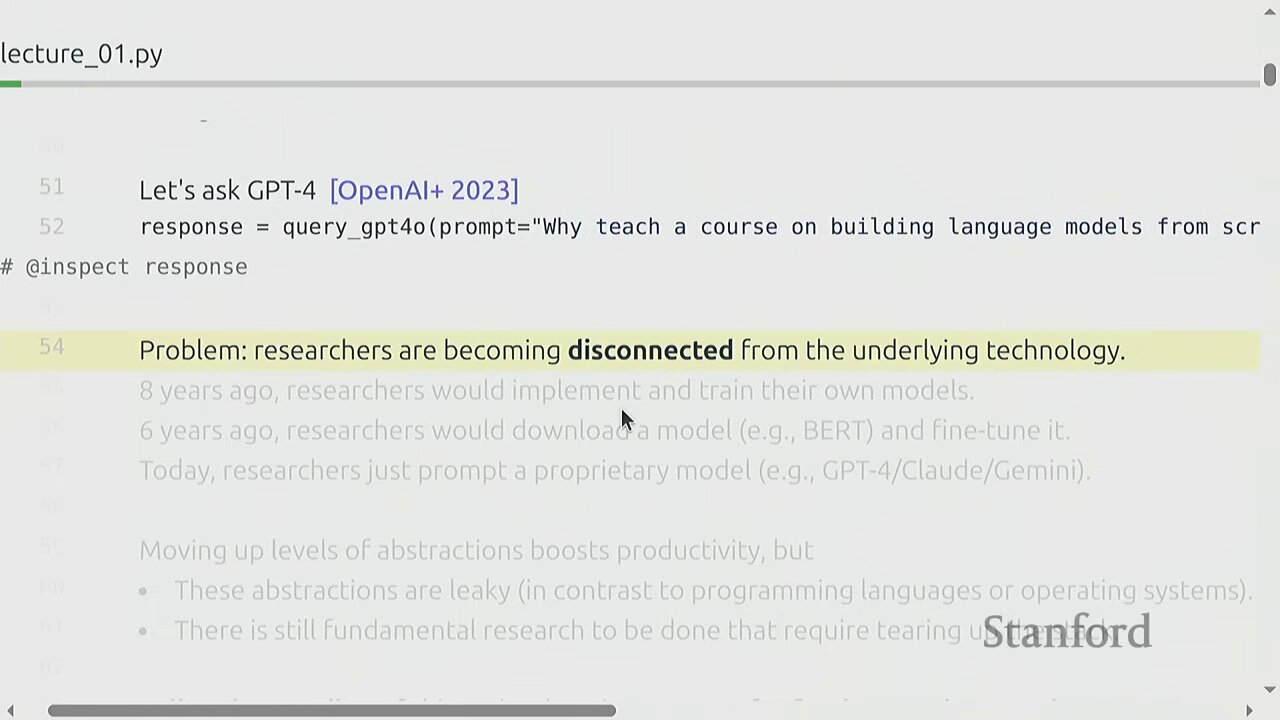
\includegraphics[width=\textwidth]{figures/fig_01_crisis.jpg}
\caption{课程动机：研究者与底层技术日益脱节\protect\footnotemark}
\end{figure}
\footnotetext{视频画面时间区间：00:02:15--00:02:45。}

Percy 坦言，这种抽象层的引入并非全盘坏事。正因为我们能简单地 prompt 语言模型，大量研究被解锁，更多人能参与到 AI 应用中来。他自己也大量使用 prompting。但关键问题在于：

\begin{warningbox}{泄漏的抽象层}
与操作系统或编程语言不同，LLM 的抽象层是\textbf{泄漏的（leaky）}。你不真正理解抽象边界在哪里——它是"string in, string out"的黑箱。从事基础研究必须拆开整个技术栈，协同设计数据、系统和模型。
\end{warningbox}

Tatsu Hashimoto 补充了他和 Percy 开设这门课的初心：他们花了很长时间思考"什么才是真正有深度的技术内容"，最终结论是——\textbf{你必须从零构建，才能真正理解它}。这是整门课的精神基调。

\subsection{小模型能否代表大模型？}

这是本课的核心张力。课程只训得起小模型（受限于学生算力），但前沿模型如 GPT-4 传闻有 1.8 万亿参数、训练成本一亿美元。这个差距带来了一个严肃的学术问题：小规模上学到的知识，能否迁移到大规模？

Percy 给出了两个具体例子说明这种 representative gap：

\begin{importantbox}{FLOPs 分布的变化}
在小模型中，Attention 层和 MLP 层消耗的 FLOPs 大致相当（约 1:1）。但到了 1750 亿参数的模型，MLP 层的 FLOPs 占绝对主导。如果你在小规模上花费大量时间优化 Attention，可能优化错了对象——大规模时它的占比已被 MLP 淹没。
\end{importantbox}

第二个例子更加微妙——\textbf{涌现能力（emergent behavior）}。Jason Wei 等人 2022 年的论文展示了一个关键现象：当你逐渐增加训练 FLOPs 时，许多任务（如 in-context learning）的准确度长期看起来毫无变化，然后突然在某一个 scale 出现跳跃式提升。如果你只在低于这个阈值的 scale 上做实验，会得出"语言模型不行"的错误结论。

\subsection{三类知识：你能拿走多少？}

面对上述 representative gap，Percy 定义了三类知识，明确了课程的预期管理：

\begin{figure}[H]
\centering
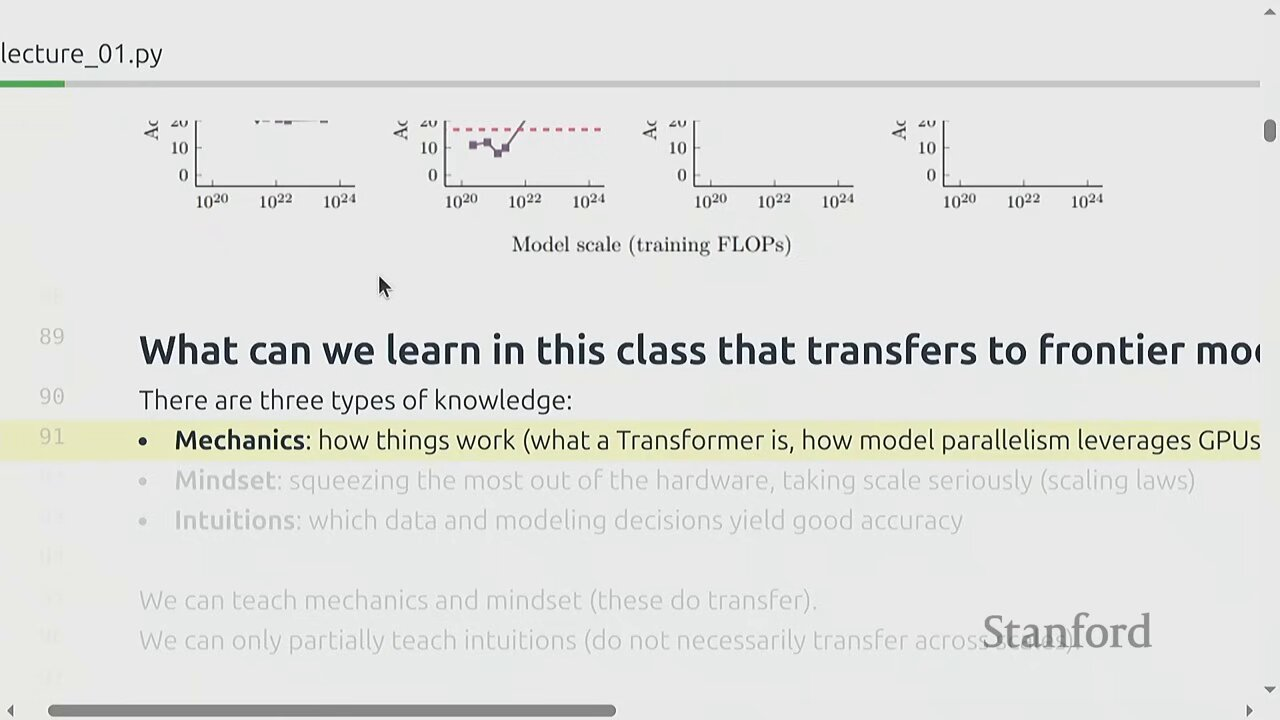
\includegraphics[width=\textwidth]{figures/fig_02_three_knowledges.jpg}
\caption{三类知识：机制、心态、直觉——课程能教你多少？\protect\footnotemark}
\end{figure}
\footnotetext{视频画面时间区间：00:07:15--00:07:45。}

\begin{tabular}{p{3cm}p{2cm}p{8cm}}
\toprule
\textbf{知识类型} & \textbf{能否教} & \textbf{说明} \\
\midrule
机制（Mechanics） & ✅ 能 & Transformer 怎么算、模型并行怎么用——这是可传授的"原料" \\
心态（Mindset） & ✅ 能 & 极致压榨硬件、严肃对待 scaling——OpenAI 凭这个杀出来 \\
直觉（Intuition） & ⚠️ 部分 & 哪些数据/架构决策有效——因为随 scale 变化，只能教一半 \\
\bottomrule
\end{tabular}

\vspace{0.3cm}

\begin{knowledgebox}{预期管理}
Percy 原话："你能拿走 2.5 / 3，已经物超所值。"这意味着课程明确承认无法教你全部的"直觉"——因为小规模有效的决策未必在大规模有效。但机制和心态是完整可迁移的。
\end{knowledgebox}

\subsection{Bitter Lesson 的正确读法}

\begin{figure}[H]
\centering
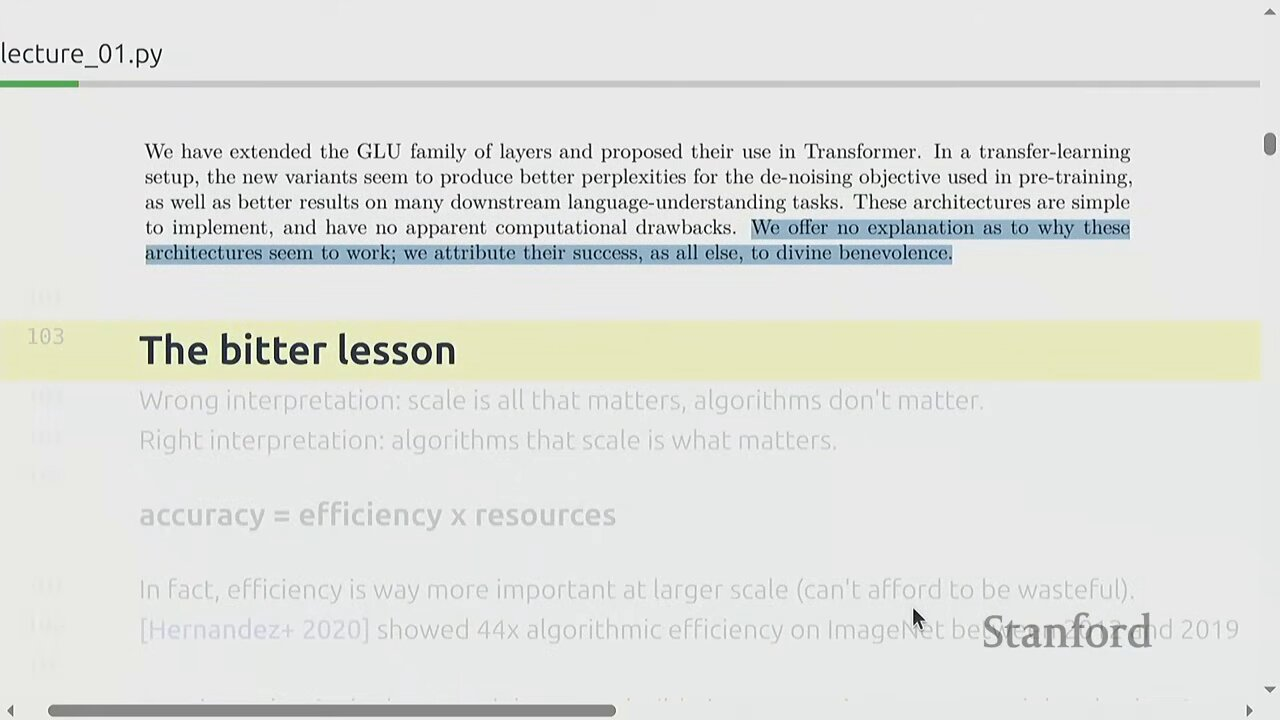
\includegraphics[width=\textwidth]{figures/fig_03_bitter_lesson.jpg}
\caption{Bitter Lesson 的两种解读\protect\footnotemark}
\end{figure}
\footnotetext{视频画面时间区间：00:09:35--00:10:05。}

Rich Sutton 的 "Bitter Lesson" 是 AI 领域被广泛引用的文章。Percy 指出了一个常见误读和正确读法：

\begin{warningbox}{常见误读}
Bitter Lesson = scale 决定一切，算法不重要，只要砸钱就行。
\end{warningbox}

\begin{importantbox}{正确读法}
算法\textbf{在 scale 下}才重要。模型质量是效率与资源的乘积：

\[
\text{accuracy} \propto \text{efficiency} \times \text{resources}
\]

\begin{itemize}
\item $\text{accuracy}$：模型在任务上的表现（如 accuracy、perplexity）
\item $\text{efficiency}$：硬件利用率和算法效率的综合
\item $\text{resources}$：投入的算力（FLOPs）和数据量（tokens）
\end{itemize}

效率在大规模下\textbf{更重要}——烧一亿美元时，你不能容忍任何浪费。
\end{importantbox}

\begin{itemize}
\item $accuracy$：模型在任务上的表现
\item $efficiency$：硬件和算法的综合效率
\item $resources$：投入的算力和数据量
\end{itemize}

实证支撑：OpenAI 2020 年的论文显示，2012 到 2019 年间，ImageNet 训练的\textbf{算法效率提升了 44 倍}，比摩尔定律还快。如果没有这些算法进步，你需要付出 44 倍的成本。

\begin{figure}[H]
\centering
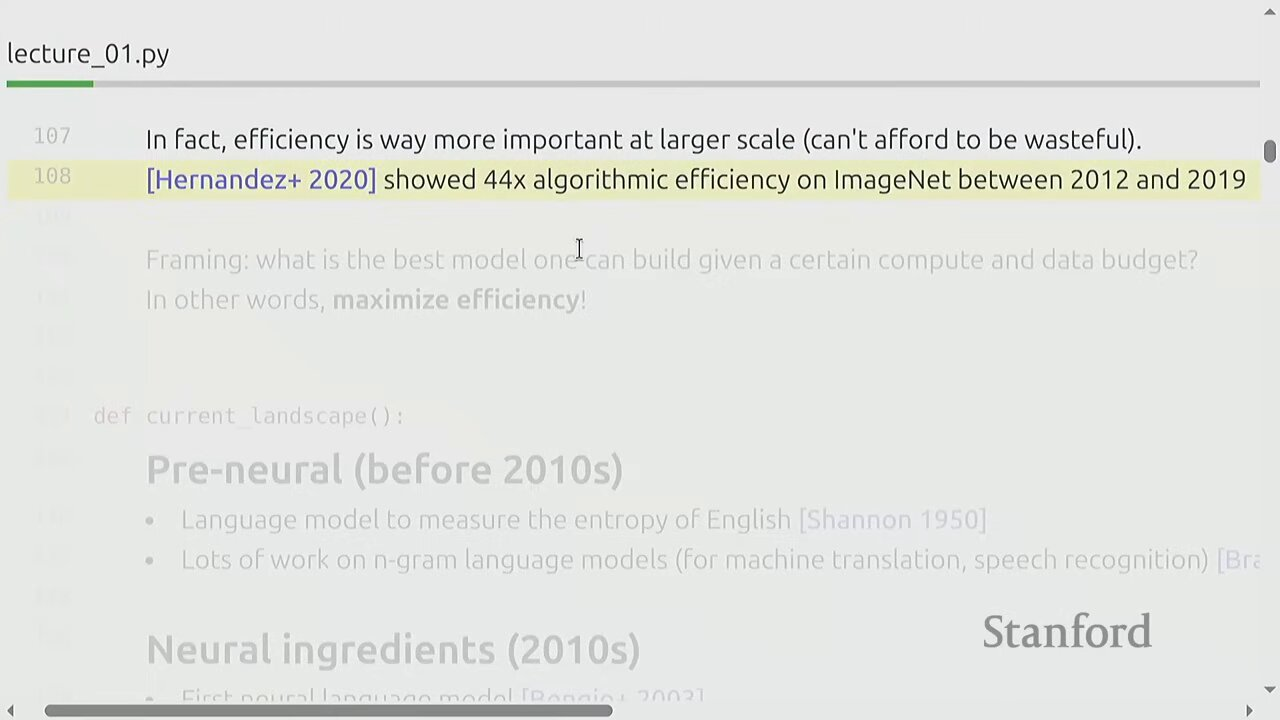
\includegraphics[width=\textwidth]{figures/fig_04_efficiency_44x.jpg}
\caption{算法效率 44 倍提升（OpenAI 2020）\protect\footnotemark}
\end{figure}
\footnotetext{视频画面时间区间：00:11:20--00:11:50。}

因此课程的核心问题可以精确表述为：

\begin{importantbox}{课程核心问题}
给定固定的 compute + data 预算，你能训练出的\textbf{最好模型}是什么？这个问题在任何 scale 下都有意义。作为研究者，我们的目标是提升算法效率。
\end{importantbox}

\subsection{本章小结}

本节确立了课程的认识论基础：LLM 的抽象层是泄漏的，基础研究需要拆栈；小模型虽不能完全代表大模型，但能可靠地传授机制与心态；Bitter Lesson 的真正教训是"算法在 scale 下重要"，效率是核心。

\section{语言模型简史}

\subsection{关键里程碑}

\begin{figure}[H]
\centering
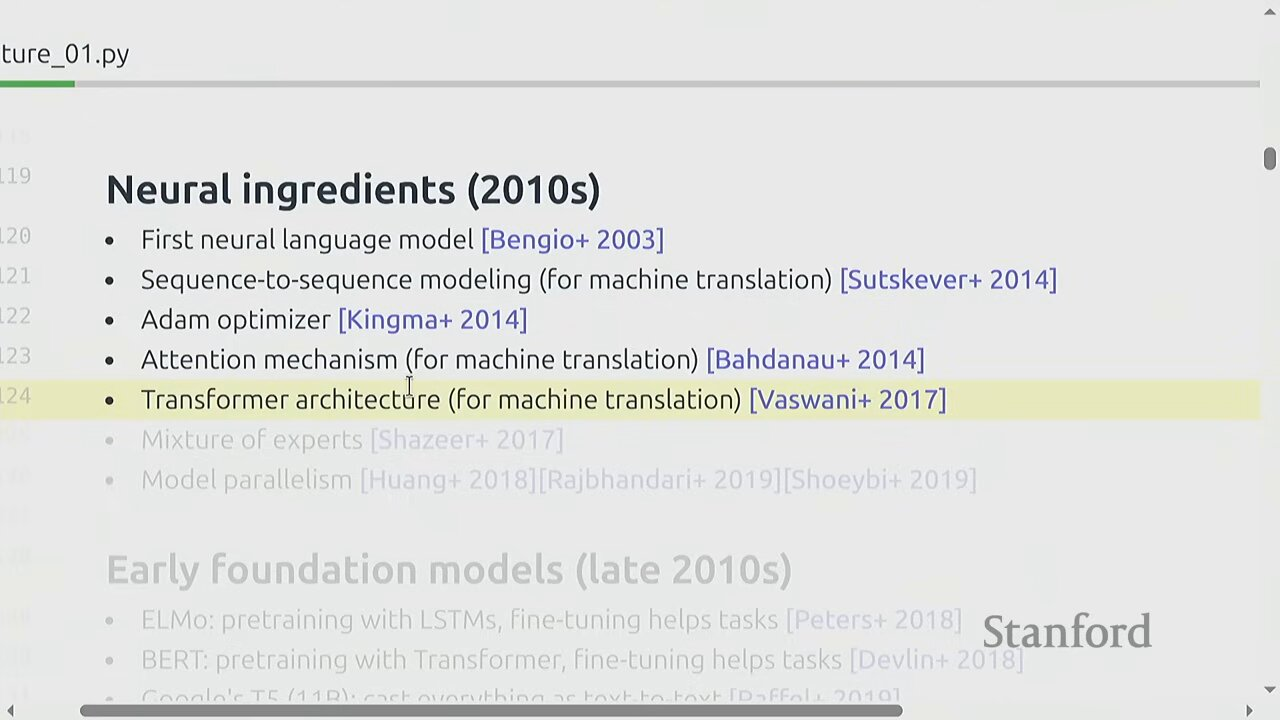
\includegraphics[width=\textwidth]{figures/fig_05_neural_ingredients.jpg}
\caption{2010 年代神经网络关键组件的时间线\protect\footnotemark}
\end{figure}
\footnotetext{视频画面时间区间：00:14:05--00:14:35。}

\begin{figure}[H]
\centering
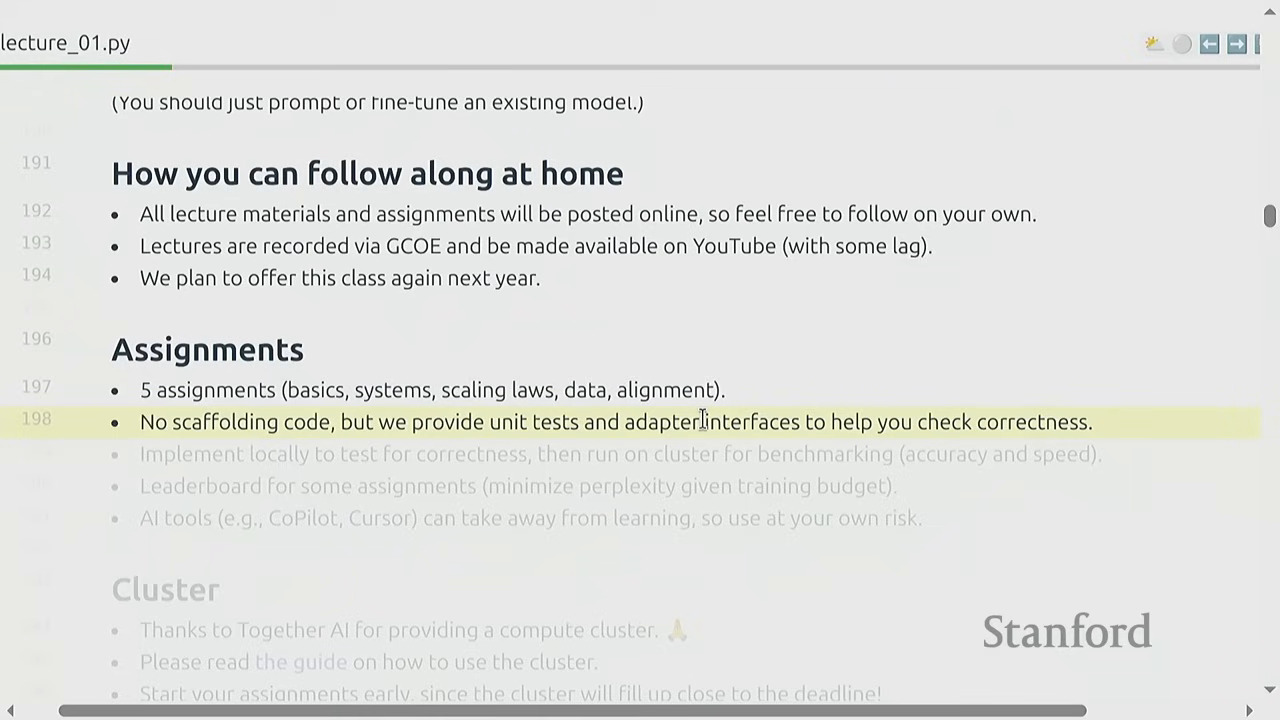
\includegraphics[width=\textwidth]{figures/fig_19_course_structure.jpg}
\caption{课程结构：五大模块的对应关系与 assignment 安排\protect\footnotemark}
\end{figure}
\footnotetext{视频画面时间区间：00:24:15--00:24:45。}

Percy 强调，Transformer 的所有核心原料在 2020 年前已经就位。理解这段历史有助于认识到：GPT 的成功并非凭空出现，而是长期技术积累加上 scaling 心态的产物。从 Bengio 2003 年的神经语言模型，到 Sutskever 的序列到序列模型，再到 Adam 优化器，每一块拼图都在为 2017 年 Transformer 的诞生铺路。而 OpenAI 的独特贡献，不在于发明了任何一个组件，而在于坚定地拥抱 scaling laws，将工程执行力和技术信仰结合，推出了 GPT 系列模型。

\begin{tabular}{p{2.5cm}p{11cm}}
\toprule
\textbf{年代} & \textbf{里程碑} \\
\midrule
$\sim$1948 & Shannon 用语言模型估算英语的熵 \\
2003 & Bengio 团队首个\textbf{神经语言模型} \\
$\sim$2014 & Seq2seq（Ilya Sutskever 等）、Adam 优化器 \\
2017 & \textbf{Attention Is All You Need}（Transformer 诞生） \\
2018--2020 & 基础模型时代：ELMo $\to$ BERT $\to$ T5 \\
2020+ & GPT-2/GPT-3：OpenAI 拥抱 scaling laws \\
2022+ & 开放权重模型浪潮：Llama / DeepSeek / Qwen \\
\bottomrule
\end{tabular}

\begin{knowledgebox}{冷知识}
Google 在 2007 年就在 \textbf{2 万亿 token} 上训了 5-gram 模型——比 GPT-3 的 token 量还大。但因为不是神经网络，没有任何涌现能力。Token 数量不是万能的，模型架构同样关键。
\end{knowledgebox}

\subsection{开放性的三个层级}

\begin{figure}[H]
\centering
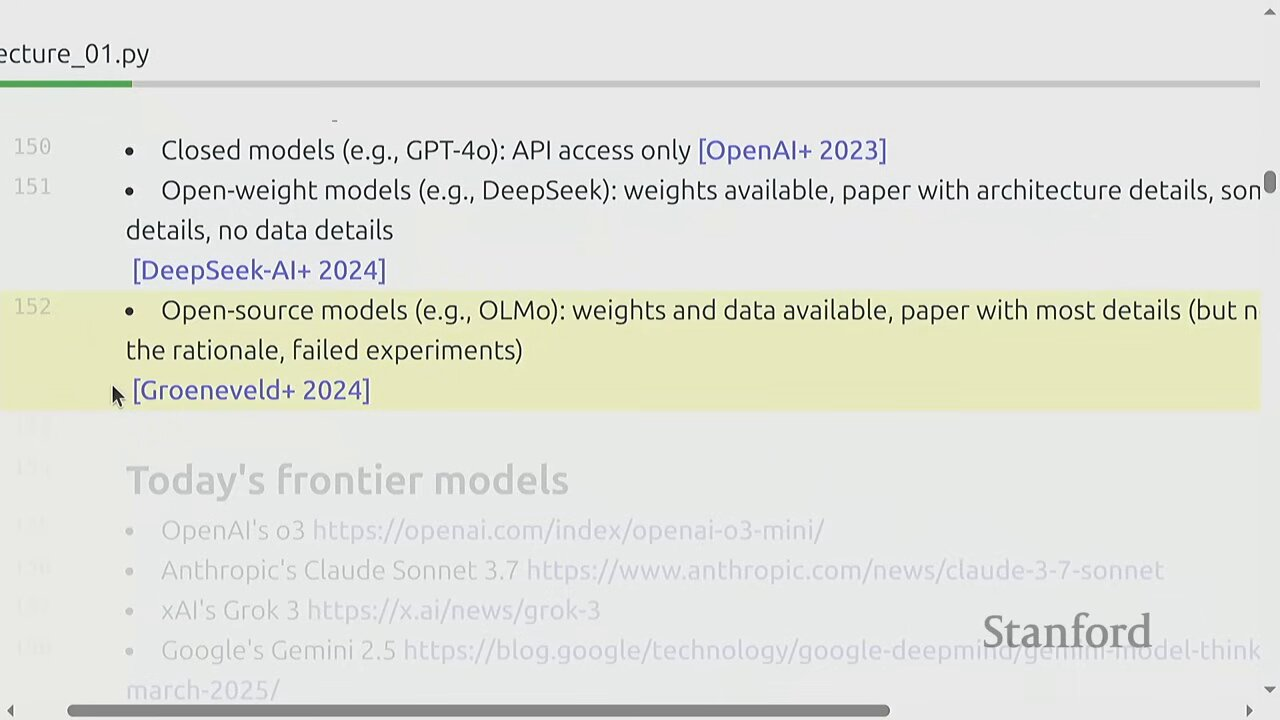
\includegraphics[width=\textwidth]{figures/fig_06_openness_levels.jpg}
\caption{模型开放性的三个层级\protect\footnotemark}
\end{figure}
\footnotetext{视频画面时间区间：00:17:00--00:17:30。}

\begin{tabular}{p{2.5cm}p{4cm}p{7cm}}
\toprule
\textbf{层级} & \textbf{例子} & \textbf{你能拿到什么} \\
\midrule
Closed & GPT-4 & 只能 API 调用，零细节 \\
Open weight & Llama & 权重 + 架构细节，无数据细节 \\
Open source & OLMo / DeepSeek & 权重 + 数据 + 诚实的技术报告 \\
\bottomrule
\end{tabular}

但无论多开放的论文，都\textbf{替代不了亲手构建}。这是课程存在的另一个理由。

\subsection{本章小结}

LLM 并非凭空诞生，其所有关键组件在 2020 年前已就位。OpenAI 的差异化贡献是 scaling 心态和工程执行。模型的"开放"分多个层级，但任何文档都无法替代亲手实现的体验。

\section{五大模块总览}

\begin{figure}[H]
\centering
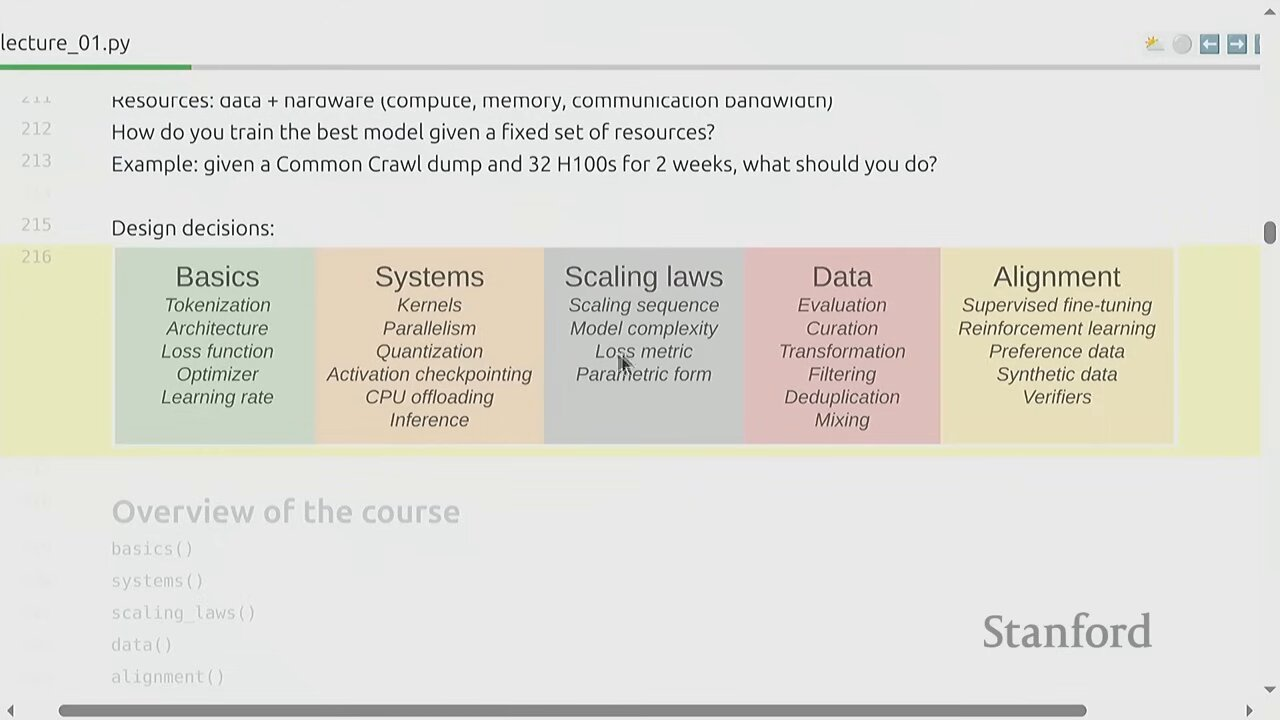
\includegraphics[width=\textwidth]{figures/fig_07_five_modules.jpg}
\caption{给定 Common Crawl + 32 块 H100 + 两周，你怎么训模型？五大模块是五类设计决策\protect\footnotemark}
\end{figure}
\footnotetext{视频画面时间区间：00:26:55--00:27:25。}

课程将"如何训练语言模型"拆解为五个相互关联的模块，对应五个 assignment。

\subsection{模块一：Basics（A1）——跑通完整管线}

目标：实现一条端到端的训练管线。

\begin{tabular}{p{2.5cm}p{5cm}p{6cm}}
\toprule
\textbf{组件} & \textbf{你要实现的} & \textbf{关键决策} \\
\midrule
Tokenizer & BPE（从零实现） & 字符串$\to$整数 \\
模型架构 & Transformer & 激活函数、位置编码、归一化 \\
训练 & Cross-entropy + AdamW & 学习率、batch size \\
\bottomrule
\end{tabular}

\begin{figure}[H]
\centering
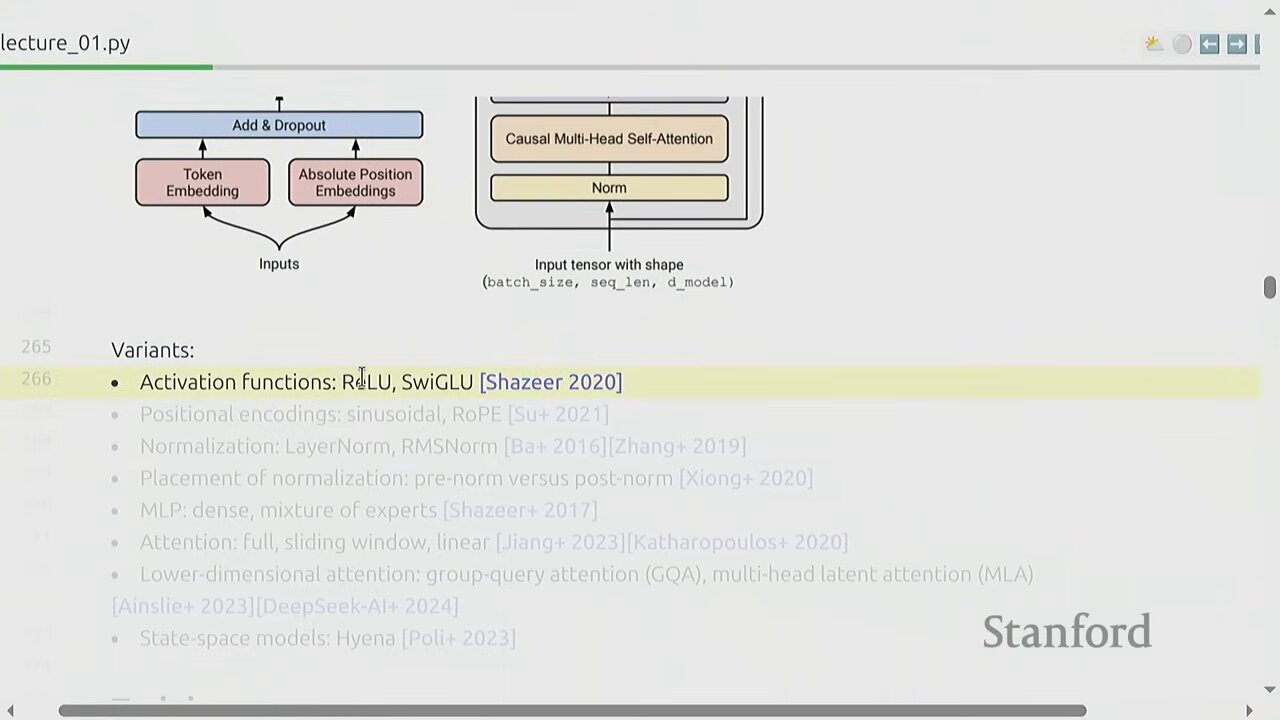
\includegraphics[width=\textwidth]{figures/fig_08_transformer_variants.jpg}
\caption{Transformer 自 2017 年以来的架构改进清单\protect\footnotemark}
\end{figure}
\footnotetext{视频画面时间区间：00:29:55--00:30:25。}

Transformer 自 2017 年诞生以来有很多"小改进"，累积起来差异巨大：

\begin{itemize}
\item \textbf{激活函数}：ReLU $\to$ SwiGLU。noam 论文原话："we offer no explanation except divine benevolence"（除了神意，我们给不出解释）。
\item \textbf{位置编码}：绝对 $\to$ RoPE（Rotary Position Embedding）
\item \textbf{归一化}：LayerNorm $\to$ RMSNorm；放置位置从 post-norm $\to$ pre-norm
\item \textbf{MLP}：dense $\to$ Mixture of Experts
\item \textbf{Attention}：full $\to$ sliding window / linear / GQA / MLA
\item \textbf{替代架构}：SSM（如 Hyena），或 hybrid 模型
\end{itemize}

原始 Attention 的计算复杂度为：

\[
\text{Attention}(Q, K, V) = \text{softmax}\left(\frac{QK^T}{\sqrt{d_k}}\right) V
\]

\begin{itemize}
\item $Q, K, V$：查询、键、值矩阵，形状为 $(L, d_k)$，其中 $L$ 为序列长度
\item $d_k$：key 的维度，$\sqrt{d_k}$ 用于缩放防止梯度消失
\item 计算和内存复杂度均为 $O(L^2 d_k)$，这是长序列的核心瓶颈
\end{itemize}

RMSNorm 相比 LayerNorm 更简单，去掉了均值减法：

\[
\text{RMSNorm}(x) = \frac{x}{\sqrt{\frac{1}{d}\sum_{i=1}^{d} x_i^2 + \epsilon}} \cdot \gamma
\]

\begin{itemize}
\item $x \in \mathbb{R}^d$：输入向量
\item $\gamma \in \mathbb{R}^d$：可学习的缩放参数
\item $\epsilon$：防止除零的小常数
\item 相比 LayerNorm 省去了均值计算 $\mu = \frac{1}{d}\sum x_i$，效率更高
\end{itemize}

\begin{figure}[H]
\centering
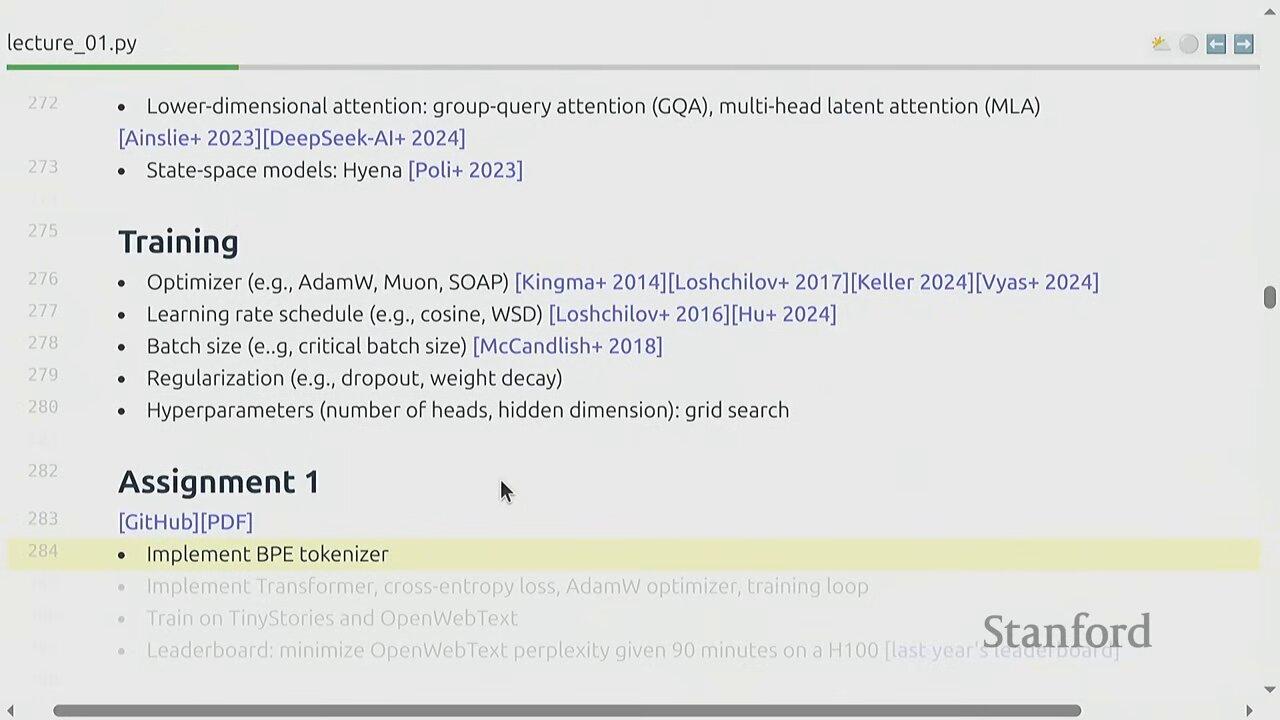
\includegraphics[width=\textwidth]{figures/fig_09_assignment1.jpg}
\caption{Assignment 1 细节：TinyStories + OpenWebText，leaderboard 是 90 分钟 H100 内最小化 perplexity\protect\footnotemark}
\end{figure}
\footnotetext{视频画面时间区间：00:32:25--00:32:55。}

\begin{warningbox}{Percy 的警告}
BPE tokenizer 是 A1 里最出人意料的重活。很多学生在这里花费大量时间。不要低估它。
\end{warningbox}

训练管线中的核心是 cross-entropy loss。给定语言模型对位置 $t$ 的预测分布 $p_\theta(\cdot | x_{<t})$ 和真实 token $x_t$：

\[
\mathcal{L}_{\text{CE}} = -\frac{1}{L} \sum_{t=1}^{L} \log p_\theta(x_t | x_{<t})
\]

\begin{itemize}
\item $p_\theta(x_t | x_{<t})$：模型在参数 $\theta$ 下，给定前缀 $x_{<t}$ 预测位置 $t$ 的概率
\item $L$：序列长度
\item Perplexity（困惑度）是 cross-entropy 的指数：$\text{PPL} = \exp(\mathcal{L}_{\text{CE}})$
\end{itemize}

AdamW 优化器的参数更新规则为：

\[
m_t = \beta_1 m_{t-1} + (1-\beta_1) g_t
\]
\[
v_t = \beta_2 v_{t-1} + (1-\beta_2) g_t^2
\]
\[
\theta_t = \theta_{t-1} - \eta \left( \frac{\hat{m}_t}{\sqrt{\hat{v}_t} + \epsilon} + \lambda \theta_{t-1} \right)
\]

\begin{itemize}
\item $m_t, v_t$：一阶矩和二阶矩估计
\item $\hat{m}_t, \hat{v}_t$：偏差修正后的矩估计
\item $\lambda$：解耦的 weight decay 系数（不进入梯度，直接作用参数）
\item $\beta_1=0.9, \beta_2=0.999$：默认衰减率
\end{itemize}

\subsection{模块二：Systems（A2）——榨取硬件性能}

\begin{figure}[H]
\centering
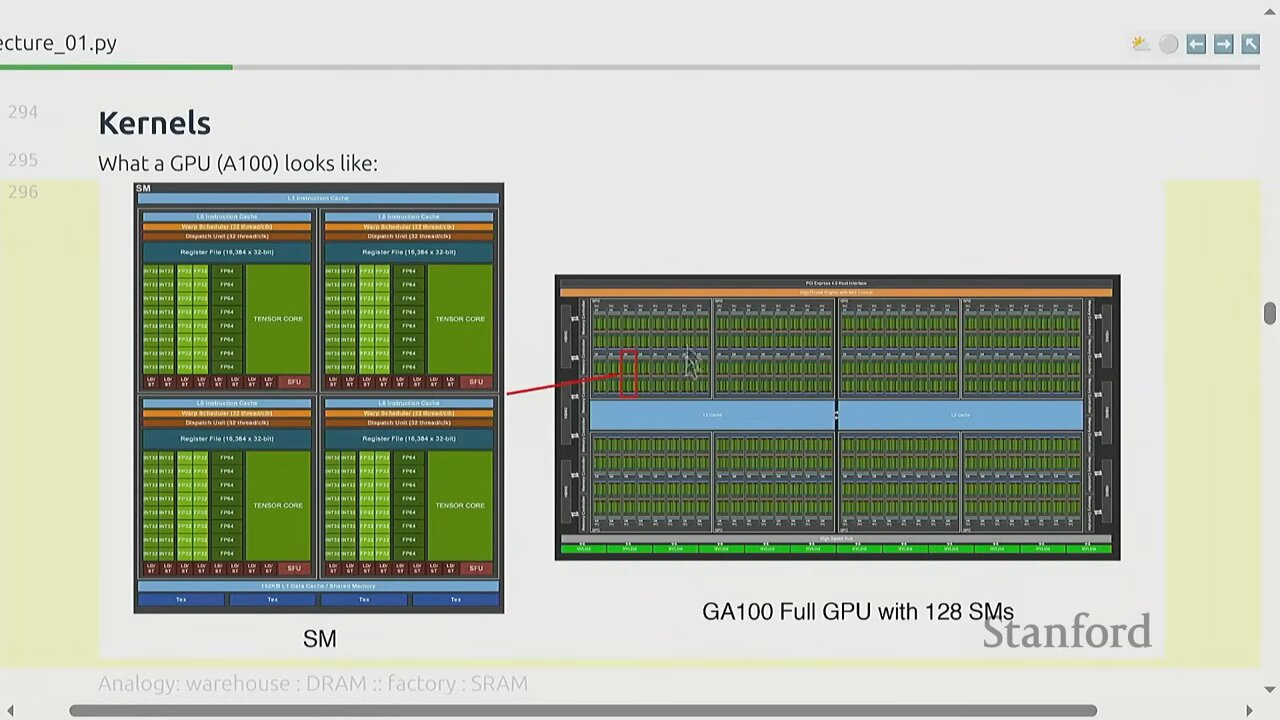
\includegraphics[width=\textwidth]{figures/fig_10_gpu_arch.jpg}
\caption{GPU 架构：浮点运算阵列 + 分层内存\protect\footnotemark}
\end{figure}
\footnotetext{视频画面时间区间：00:34:25--00:34:55。}

核心目标：从硬件中榨取最大性能。

\textbf{Kernel（单 GPU）}：GPU 本质上是一个庞大的浮点运算阵列，配备分层内存（L2/L1 cache 在芯片上，HBM 在芯片外）。

\begin{figure}[H]
\centering
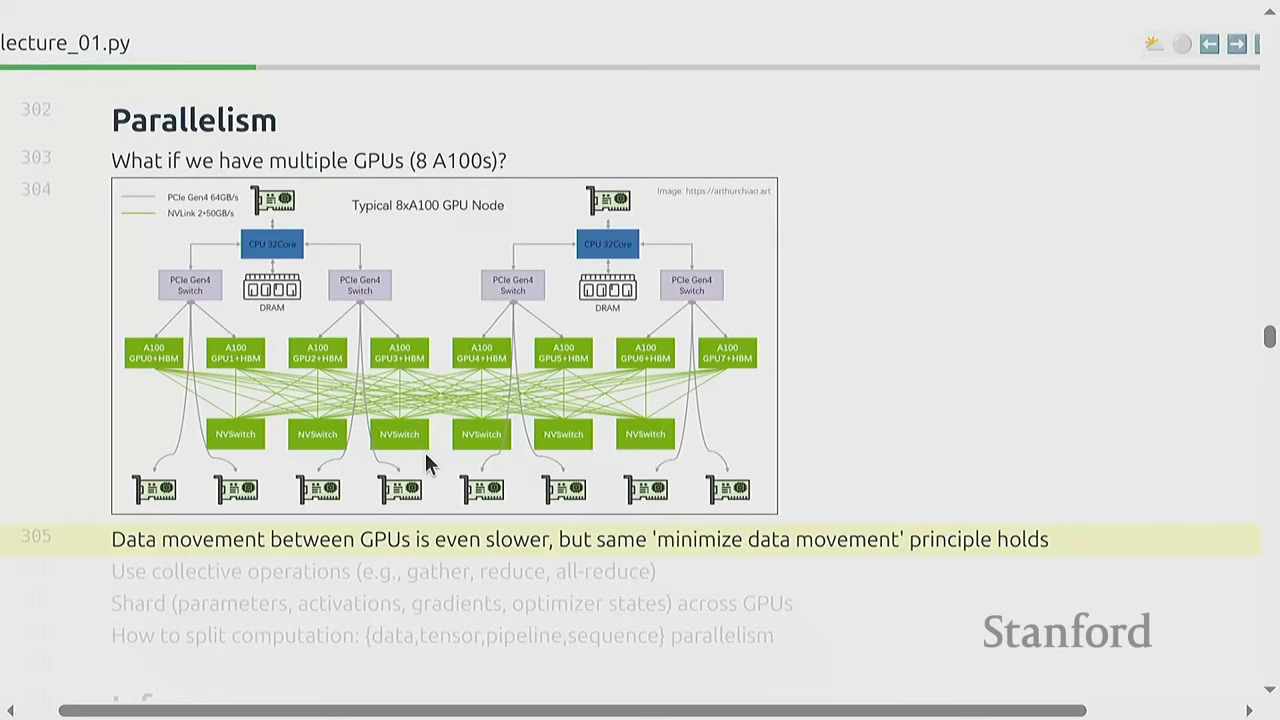
\includegraphics[width=\textwidth]{figures/fig_20_triton_kernels.jpg}
\caption{Triton kernel：用 Python 写 GPU kernel，自动 tile/block\protect\footnotemark}
\end{figure}
\footnotetext{视频画面时间区间：00:36:15--00:36:45。}

\begin{knowledgebox}{仓库-工厂类比}
内存是仓库（存放数据和模型参数），计算是工厂（执行运算）。瓶颈不在工厂的产能，而在\textbf{搬运成本（data movement）}。优化目标：用 fusion（算子融合）、tiling（分块）等技术最小化数据搬运。

模型训练的 FLOPs 利用率（MFU）是衡量系统效率的关键指标：

\[
\text{MFU} = \frac{\text{实际 FLOPs/s}}{\text{GPU 理论峰值 FLOPs/s}}
\]

好的实现能达到 50\% 以上，差的实现可能只有 5\%。这意味着同样的硬件预算，效率差距可以达到 10 倍。

训练单个模型的总耗时可以用以下公式粗略估算。给定模型参数量 $N$、训练 token 数 $D$、GPU 数量 $G$、单卡峰值算力 $P$、MFU 为 $\eta$：

\[
T_{\text{train}} = \frac{6 \cdot N \cdot D}{G \cdot P \cdot \eta}
\]

\begin{itemize}
\item $T_{\text{train}}$：总训练时间（秒）
\item 分子 $6ND$：总训练 FLOPs（前向 2 + 反向 4）
\item 分母 $G \cdot P \cdot \eta$：GPU 集群的实际吞吐量
\item 例：1.4B 模型训 28B token，用 32 块 H100（$P \approx 989$ TFLOPS，$\eta = 0.4$），约需 4.6 小时
\end{itemize}
\end{knowledgebox}

\textbf{Parallelism（多 GPU）}：从 8 卡开始变得有趣。GPU 之间通过 NVLink/NVSwitch 直连，但 GPU 间数据搬运比 GPU 内部更慢。策略包括 data parallelism（数据并行）和 tensor parallelism（张量并行，如 FSDP）。

\textbf{Inference}：分两个阶段——

\begin{figure}[H]
\centering
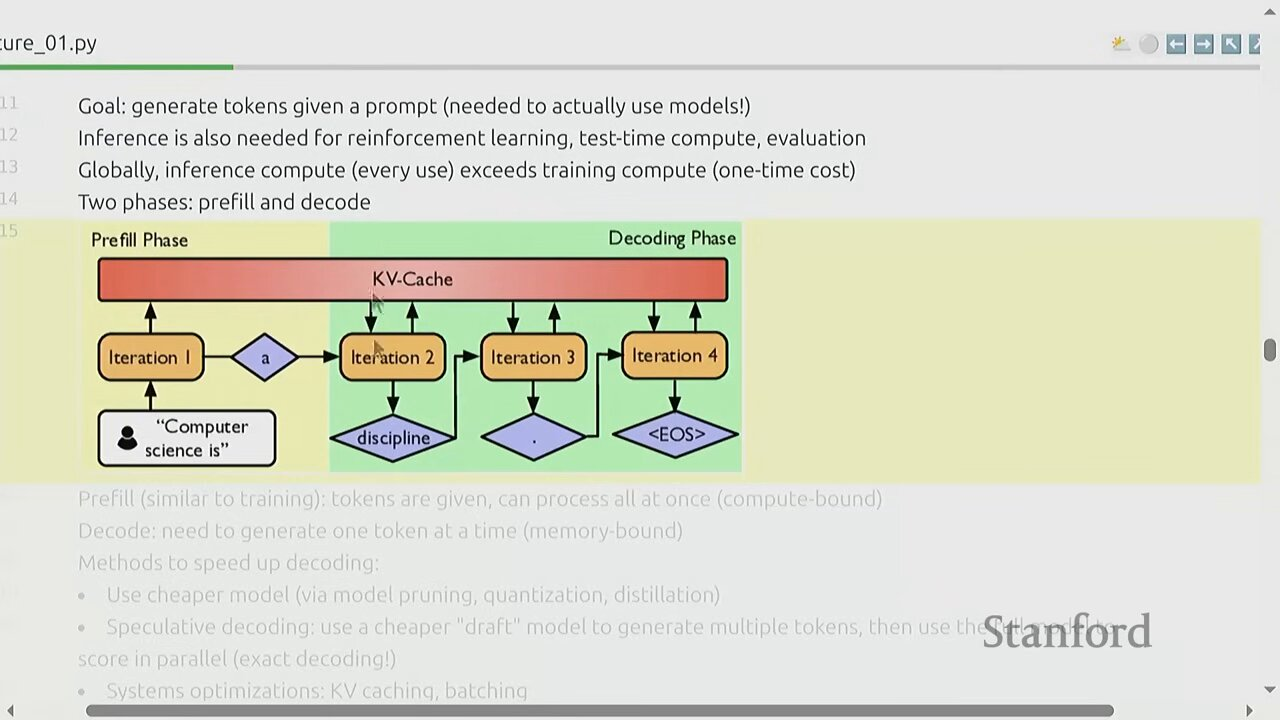
\includegraphics[width=\textwidth]{figures/fig_11_inference_phases.jpg}
\caption{推理的两阶段：prefill（并行，compute-bound）vs decode（逐 token，memory-bound）\protect\footnotemark}
\end{figure}
\footnotetext{视频画面时间区间：00:38:25--00:38:55。}

\begin{tabular}{p{2cm}p{5cm}p{6cm}}
\toprule
\textbf{阶段} & \textbf{特征} & \textbf{瓶颈} \\
\midrule
Prefill & prompt 一次性灌入，天然并行 & compute-bound \\
Decode & 自回归逐 token 生成 & memory-bound，难饱和 GPU \\
\bottomrule
\end{tabular}

\begin{importantbox}{推理经济学}
推理成本正超越训练成本——训练是一次性的，推理随用量线性增长。因此推理效率极其重要。加速手段包括：用更便宜的模型、speculative decoding（小模型探路、大模型批量验收）。
\end{importantbox}

\subsection{模块三：Scaling Laws（A3）——小规模实验，大规模预测}

\begin{figure}[H]
\centering
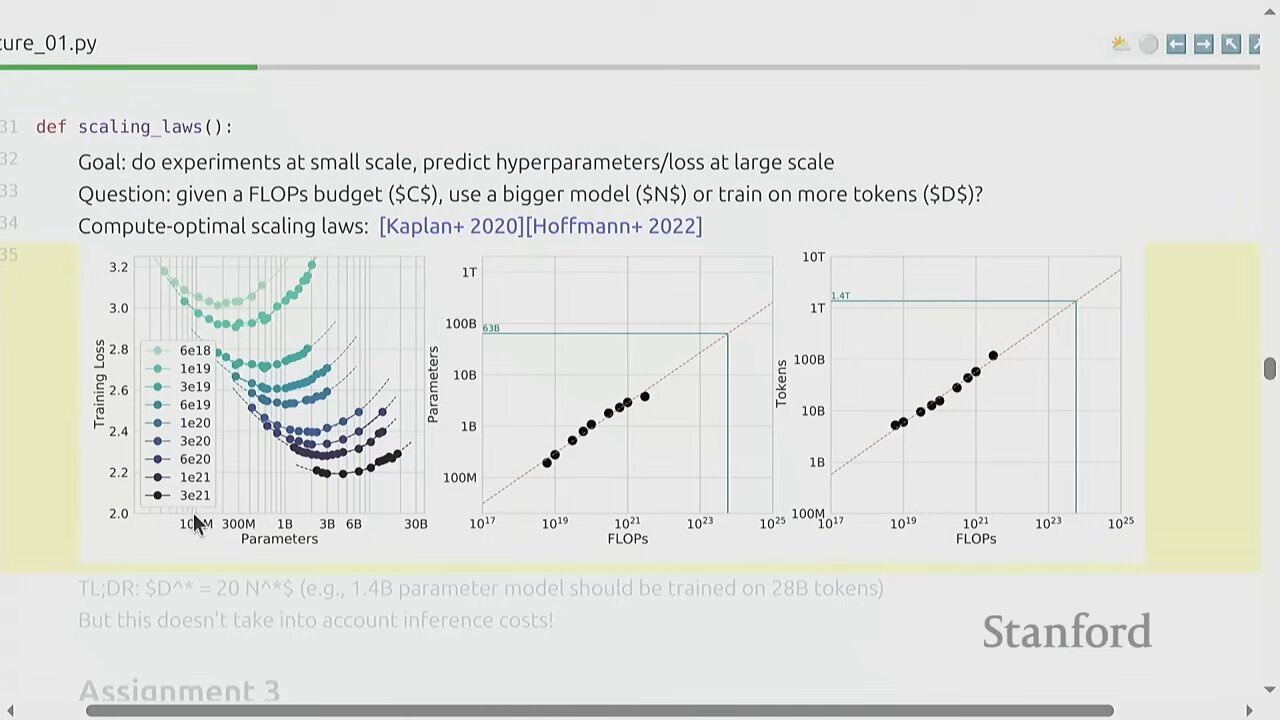
\includegraphics[width=\textwidth]{figures/fig_12_scaling_laws.jpg}
\caption{Scaling laws：每个 FLOPs 预算有一个最优 (params, data) 组合\protect\footnotemark}
\end{figure}
\footnotetext{视频画面时间区间：00:41:55--00:42:25。}

\textbf{核心问题}：给你一个 FLOPs 预算，模型该多大？大模型 = 少数据；小模型 = 多数据。最佳配比是什么？

\begin{importantbox}{Chinchilla 最优}
每个参数约配 \textbf{20 个 token}。

\[
N_{\text{tokens}}^{\text{optimal}} \approx 20 \times N_{\text{params}}
\]

\begin{itemize}
\item $N_{\text{tokens}}^{\text{optimal}}$：给定 compute 预算下的最优训练 token 数
\item $N_{\text{params}}$：模型参数量
\end{itemize}

例：1.4B 模型应训 28B token。

训练总计算量（FLOPs）可用以下公式估算：

\[
C \approx 6 \times N_{\text{params}} \times N_{\text{tokens}}
\]

\begin{itemize}
\item $C$：总训练 FLOPs
\item 系数 6：每个参数在每个 token 上做约 6 次 FLOPs（前向 2 + 反向 4）
\end{itemize}

代入 Chinchilla 最优比（$N_{\text{tokens}} = 20 N_{\text{params}}$）：

\[
C_{\text{optimal}} \approx 120 \, N_{\text{params}}^2
\]

这意味着 compute 预算翻倍时，最优模型参数只增长 $\sqrt{2} \approx 1.41$ 倍。
\end{importantbox}

\begin{warningbox}{Chinchilla 的局限}
Chinchilla 只优化训练 loss，\textbf{不考虑推理成本}。实际部署中，你可能愿意 over-train 一个更小的模型（更多 token），因为推理时它更便宜。这也是为什么 Llama 系列选择了 "over-train" 策略。
\end{warningbox}

A3 的特殊玩法：课程提供一个 training API，学生用超参查询 loss，在 FLOPs 预算内拟合 scaling law，预测最优 $(N_{\text{params}}, N_{\text{tokens}})$ 组合。预算用完就没了——模拟前沿实验室的真实决策压力。

\begin{figure}[H]
\centering
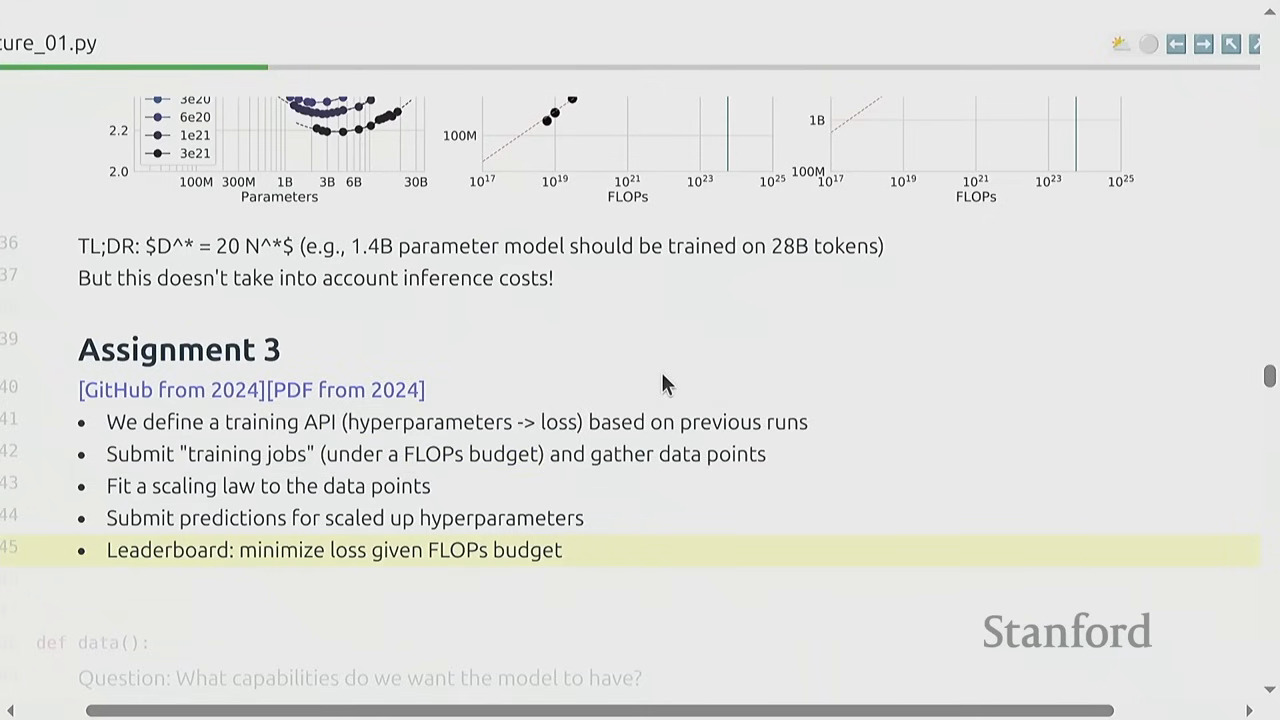
\includegraphics[width=\textwidth]{figures/fig_21_training_api.jpg}
\caption{A3 的 Training API：给定超参查询 loss，在预算内拟合 scaling law\protect\footnotemark}
\end{figure}
\footnotetext{视频画面时间区间：00:44:15--00:44:45。}

IsoFLOP 曲线是 scaling law 实验的核心方法。固定一个 compute 预算 $C$，在不同模型大小 $N$ 下训练，画出 loss 关于 $N$ 的曲线：

\[
L(N, C) = \text{loss at model size } N \text{ with compute budget } C
\]

每个 $C$ 值都有一个最优的 $N^*(C)$，连接所有最优点就得到 compute-optimal frontier。Hoffmann 等人（Chinchilla 论文）发现这个关系近似为幂律：

\[
L^*(C) \approx \alpha C^{-\beta}
\]

\begin{itemize}
\item $\alpha, \beta$：通过实验数据拟合的常数
\item $L^*(C)$：给定 compute 预算 $C$ 下的最小可达 loss
\item 这个幂律关系使我们可以从小规模实验外推大规模性能
\end{itemize}

\subsection{模块四：Data（A4）——从脏数据到训练数据}

\begin{figure}[H]
\centering
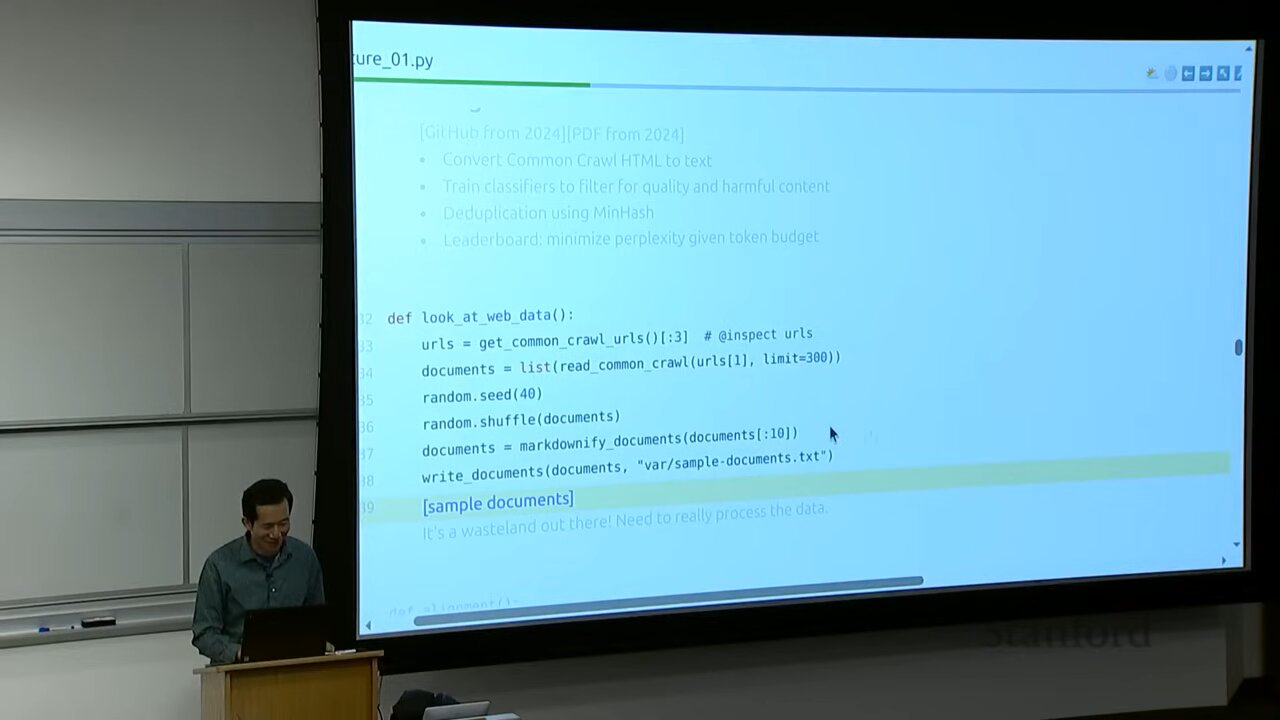
\includegraphics[width=\textwidth]{figures/fig_13_data_pipeline.jpg}
\caption{数据管线：从原始 crawl 到可训练文本\protect\footnotemark}
\end{figure}
\footnotetext{视频画面时间区间：00:46:55--00:47:25。}

\begin{warningbox}{澄清误解}
"我们在互联网上训模型"——这句话是错的。数据不会从天而降，必须\textbf{主动获取}。Percy 现场展示 Common Crawl 随机 10 篇文档：大量是垃圾、spam、非目标语言。网络比你想的脏得多。
\end{warningbox}

数据管线的完整流程：

\begin{enumerate}
\item \textbf{抓取}：crawl HTML / PDF / code directories
\item \textbf{转换}：HTML $\to$ text（有损过程！如何保留结构和内容？）
\item \textbf{质量过滤}：训分类器，区分高质量文本
\item \textbf{去重}：deduplication（MinHash 等技术）
\item \textbf{安全过滤}：移除有害内容
\end{enumerate}

\begin{knowledgebox}{数据经济学}
前沿模型现在\textbf{花钱买数据}。公开互联网的数据已不足以支撑极致性能。数据已成为新的瓶颈——行业正从 compute-constrained 走向 data-constrained。
\end{knowledgebox}

\subsection{模块五：Alignment（A5）——让 base model 有用}

\begin{figure}[H]
\centering
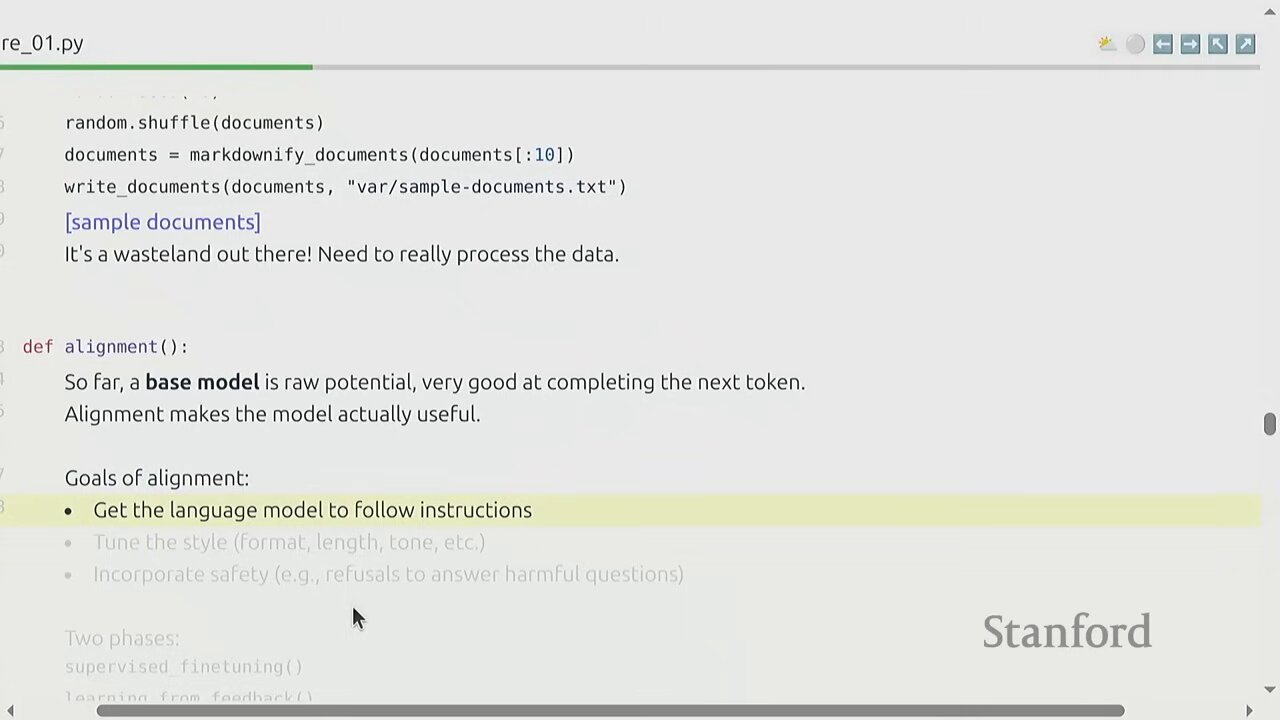
\includegraphics[width=\textwidth]{figures/fig_14_alignment.jpg}
\caption{Alignment 两阶段：SFT（监督微调）+ 学习反馈（RLHF/DPO/GRPO）\protect\footnotemark}
\end{figure}
\footnotetext{视频画面时间区间：00:50:55--00:51:25。}

Base model 只会续写下一个 token。Alignment 让它\textbf{有用}，三个维度：

\begin{tabular}{p{2.5cm}p{11cm}}
\toprule
\textbf{维度} & \textbf{目标} \\
\midrule
指令遵循 & 真正执行指令，而非续写指令文本 \\
风格控制 & 长短、格式、语气（ChatGPT vs Grok 风格不同） \\
安全 & 拒绝有害请求 \\
\bottomrule
\end{tabular}

\textbf{两阶段}：

\textbf{阶段一：SFT（Supervised Fine-Tuning）}。收集 (user, assistant) 对，监督学习。Base model 已有"原始潜力"，少量高质量样本即可解锁指令遵循。

\begin{importantbox}{LIMA 的启示}
LIMA 论文证明：\textbf{1000 条}高质量、多样化的样本就够让 base model 获得指令遵循能力。因为"对齐是浅层的"（alignment is shallow）——知识在 pretraining 已学到，alignment 只是教模型如何使用这些知识。
\end{importantbox}

\textbf{阶段二：学习反馈}。标注更轻量（偏好数据而非完整答案），算法做更多工作。

\begin{itemize}
\item \textbf{偏好数据}：生成 A/B 两个回答，人类标注哪个更好
\item \textbf{验证器}：数学/代码有形式验证；或训一个 reward model
\item \textbf{算法演进}：PPO $\to$ DPO（只需偏好数据，更简单）$\to$ GRPO（DeepSeek 开发，去掉了 value function 的 PPO 变体）
\end{itemize}

\begin{figure}[H]
\centering
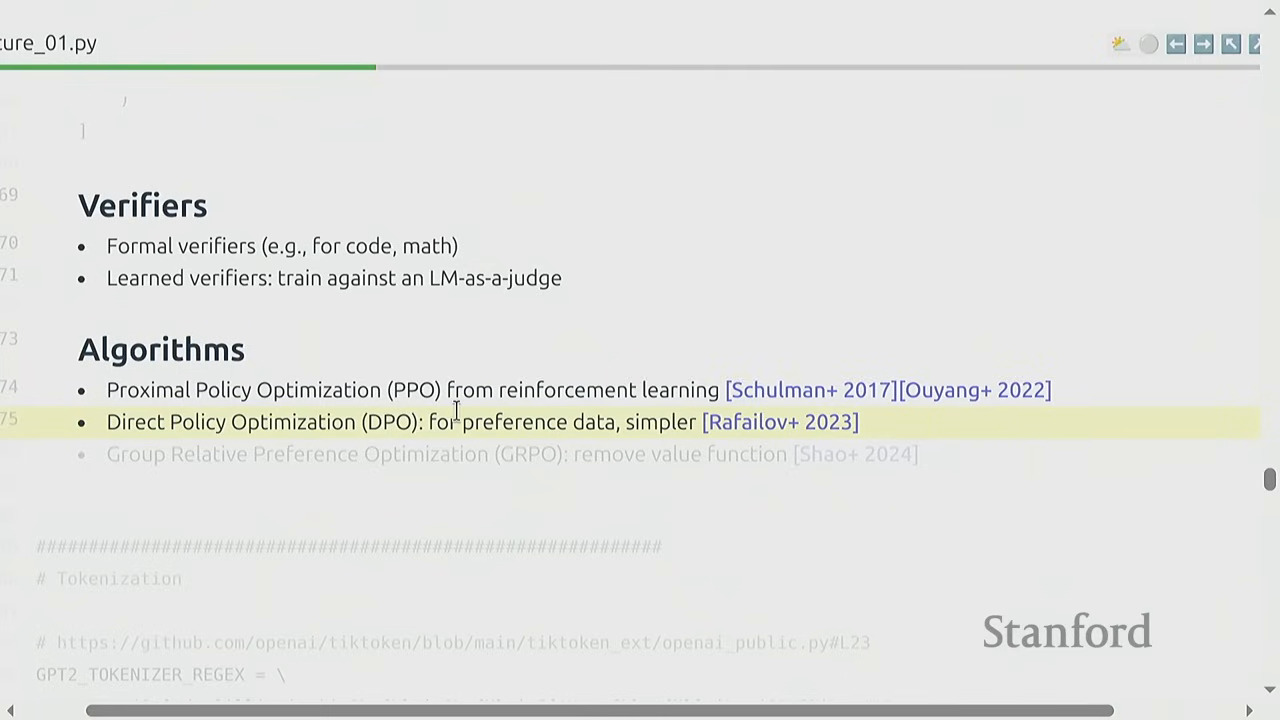
\includegraphics[width=\textwidth]{figures/fig_22_alignment_algorithms.jpg}
\caption{对齐算法对比：PPO / DPO / GRPO 的训练流程差异\protect\footnotemark}
\end{figure}
\footnotetext{视频画面时间区间：00:54:15--00:54:45。}

DPO 的核心优势在于直接从偏好数据学习，无需训练 reward model。其目标函数为：

\[
\mathcal{L}_{\text{DPO}} = -\log \sigma\left(\beta \log \frac{\pi_\theta(y_w|x)}{\pi_{\text{ref}}(y_w|x)} - \beta \log \frac{\pi_\theta(y_l|x)}{\pi_{\text{ref}}(y_l|x)}\right)
\]

\begin{itemize}
\item $\pi_\theta$：当前训练的策略（policy）
\item $\pi_{\text{ref}}$：参考策略（通常是 SFT 后的模型，固定不变）
\item $y_w, y_l$：偏好对中的获胜（winning）和落败（losing）回答
\item $\sigma$：sigmoid 函数
\item $\beta$：控制偏离参考模型的强度
\end{itemize}

\subsection{本章小结}

五大模块覆盖了语言建模的完整技术栈。Basics 建立基础管线，Systems 优化硬件利用，Scaling Laws 指导资源分配，Data 处理训练燃料，Alignment 让模型有用。每个模块都对应一个从零实现的 assignment。

\section{效率作为统一视角}

\begin{figure}[H]
\centering
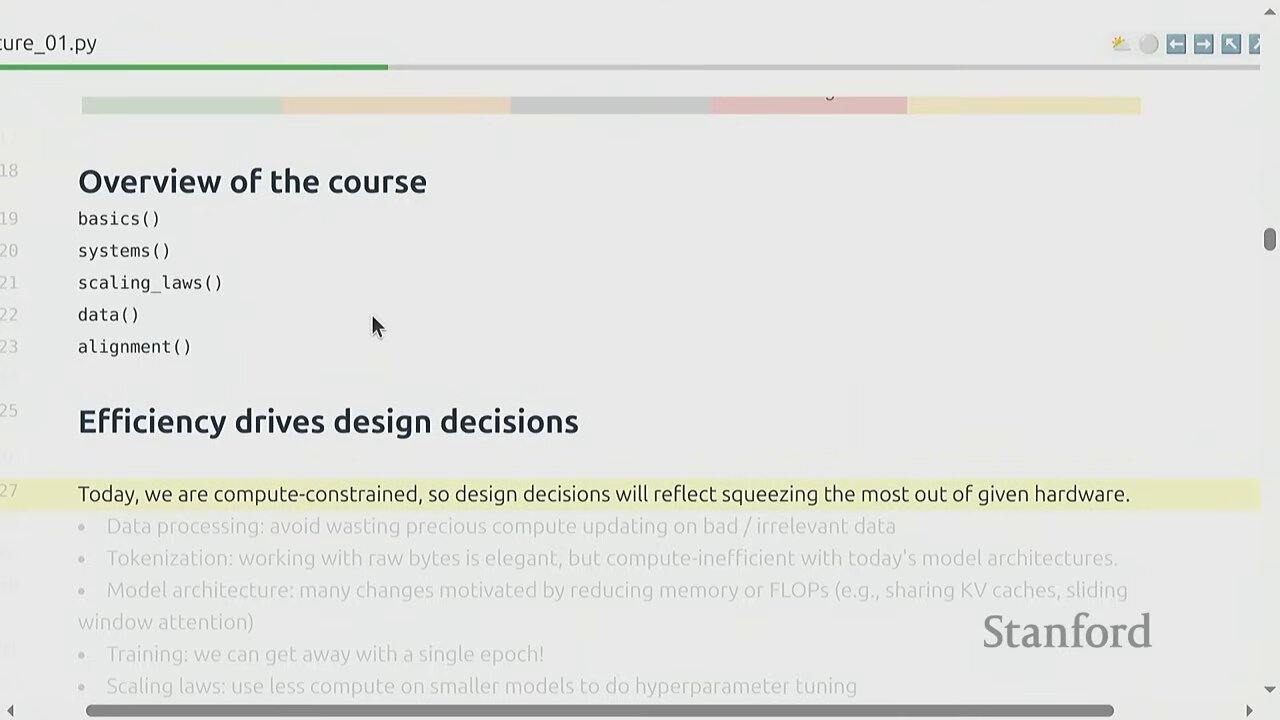
\includegraphics[width=\textwidth]{figures/fig_15_efficiency_unify.jpg}
\caption{效率作为统一主线：compute-constrained regime 下的设计决策\protect\footnotemark}
\end{figure}
\footnotetext{视频画面时间区间：00:56:15--00:56:45。}

\begin{importantbox}{贯穿五模块的主线}
我们处于 \textbf{compute-constrained} regime（算力受限）。所有设计决策都源于"压榨硬件"。理解这一点，很多看似奇怪的设计选择就变得合理了。
\end{importantbox}

\begin{tabular}{p{2.5cm}p{11cm}}
\toprule
\textbf{模块} & \textbf{效率驱动的设计决策} \\
\midrule
数据 & 激进过滤——不把算力浪费在坏数据上 \\
分词 & 字节级优雅但算力浪费，BPE 是效率妥协 \\
架构 & 大量决策由计算效率驱动（如 attention 变体） \\
训练 & 单 epoch——我们赶时间，要多见数据而非多看单点 \\
Scaling laws & 用更少算力找最优超参 \\
对齐 & 算力投入对齐 $\to$ 可用更小 base model \\
\bottomrule
\end{tabular}

\begin{knowledgebox}{范式转变}
前沿实验室正从 compute-constrained 走向 \textbf{data-constrained}。到那时，设计决策会根本性改变：单 epoch 不再合理（有更多算力为何不多跑几轮？），甚至 Transformer 架构本身（本就是 compute efficiency 的产物）都可能被替代。
\end{knowledgebox}

\section{分词深入——BPE}

\subsection{分词是什么}

\begin{figure}[H]
\centering
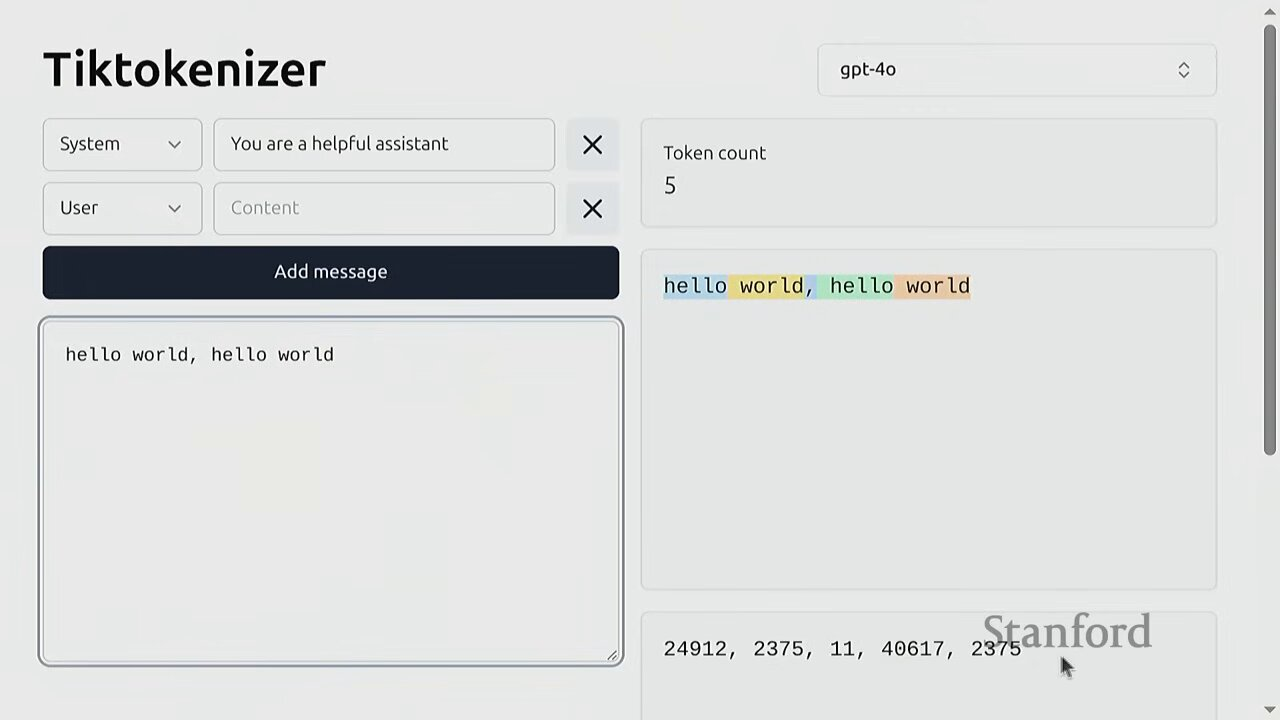
\includegraphics[width=\textwidth]{figures/fig_16_tokenizer_demo.jpg}
\caption{分词器演示：GPT-4o tokenizer 将文本切分为 token\protect\footnotemark}
\end{figure}
\footnotetext{视频画面时间区间：00:61:00--00:61:30。}

\textbf{Tokenizer} 是字符串与整数序列之间的双向映射。每个整数代表一个 token，词汇表大小（vocab size）是 token 能取的整数值范围。

\begin{importantbox}{分词的关键观察}
\begin{itemize}
\item 空格\textbf{属于} token 的一部分（" hello" $\neq$ "hello"，是两个不同 token）
\item 空格按惯例\textbf{前缀}到 token（这是 pre-tokenizer 的设计选择）
\item 数字被切成任意片段（左到右，不按千位分组）
\item 分词必须是\textbf{可逆的}（round-trip consistency）
\end{itemize}
\end{importantbox}

\subsection{四种方案的演进}

\subsubsection{方案 1：字符级（Character-based）}

每个 Unicode 字符映射到码点（code point）整数。`a` $\to$ 97，`🌍` $\to$ 127757。

\begin{warningbox}{问题}
\begin{itemize}
\item 压缩比差（每个 token 只代表少量字节）
\item 词汇表巨大（149k+ Unicode 码点）
\item 稀疏：有些字符极罕见，白白占 vocab 名额
\end{itemize}
\end{warningbox}

\subsubsection{方案 2：字节级（Byte-based）}

一切转 UTF-8 字节。词汇表固定 0--255。

\begin{figure}[H]
\centering
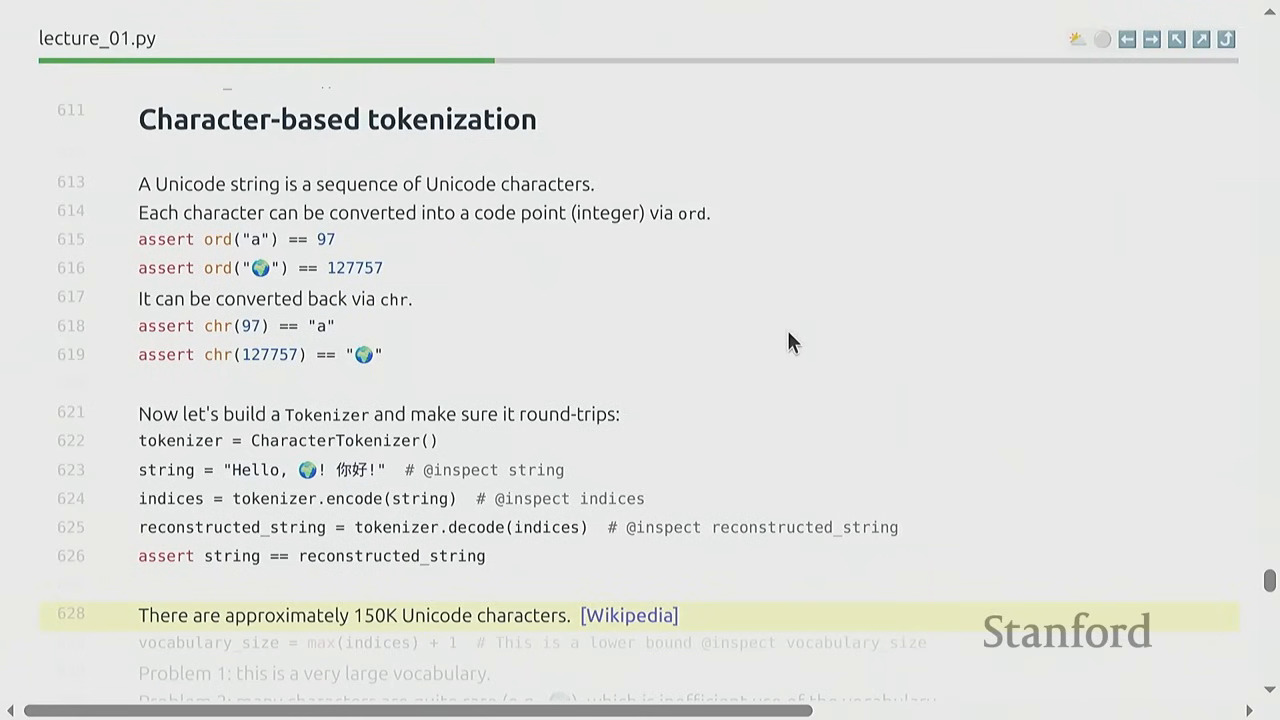
\includegraphics[width=\textwidth]{figures/fig_23_byte_tokenization.jpg}
\caption{字节级分词：每个 token 就是一个字节，压缩比为 1.0\protect\footnotemark}
\end{figure}
\footnotetext{视频画面时间区间：00:66:15--00:66:45。}

\begin{itemize}
\item ✅ 优点：vocab 小（固定 256）、无稀疏问题、任何字符串都能表示
\item ❌ \textbf{致命缺点}：压缩比 $r = 1.0$（1 byte/token）。序列太长 $\to$ attention 是 $O(N^2)$ 的，计算和内存开销灾难性增长。
\end{itemize}

具体来说，一段 1000 字节的文本，字节级分词产生 1000 个 token，而 BPE 可能只产生约 625 个（$r=1.6$）。序列长度差异导致 attention 计算量差距为 $(1000/625)^2 \approx 2.56$ 倍——这在大规模训练中是巨大的浪费。

字节级方案的 attention 计算量与 BPE 的比值为：

\[
\frac{C_{\text{byte}}}{C_{\text{BPE}}} = \frac{L_{\text{byte}}^2}{L_{\text{BPE}}^2} = \frac{1}{r^2} \approx \frac{1}{1.6^2} \approx 2.56
\]

\begin{itemize}
\item $C_{\text{byte}}, C_{\text{BPE}}$：字节级和 BPE 方案的 attention 计算量
\item $r$：BPE 的压缩比
\item 这意味着 BPE 在 attention 上节省了约 $1 - 1/2.56 \approx 61\%$ 的计算
\end{itemize}

\begin{knowledgebox}{Percy 的心声}
"我真希望 byte-level 能行，它最优雅——但今天的架构下它太慢了。"这是 efficiency 主线的直接体现。未来如果出现不依赖 $O(N^2)$ attention 的架构，byte-level 可能重新变得可行。
\end{knowledgebox}

\subsubsection{方案 3：词级（Word-based）}

用正则分词（如 GPT-2 的 pre-tokenizer regex），每个 segment 是一个 token。

\begin{warningbox}{致命缺点}
词汇表\textbf{无界}。新词不断出现，全得映射到 \texttt{<UNK>}。这导致 perplexity 计算失真，且无法处理未登录词。
\end{warningbox}

\subsubsection{方案 4：BPE（Byte Pair Encoding）✅}

\begin{importantbox}{核心洞察}
不要预设怎么切——\textbf{在原始文本上训练 tokenizer}。让频繁序列合并成一个 token，罕见序列拆成多个 token。这是\textbf{数据驱动的自适应}方案。
\end{importantbox}

\textbf{历史脉络}：Philip Gage 1994 年为数据压缩发明 BPE；2015 年 Sennrich 等将其引入神经机器翻译（替代烦人的 word-based）；GPT-2 正式带入语言建模时代。

\subsection{BPE 算法详解}

\begin{figure}[H]
\centering
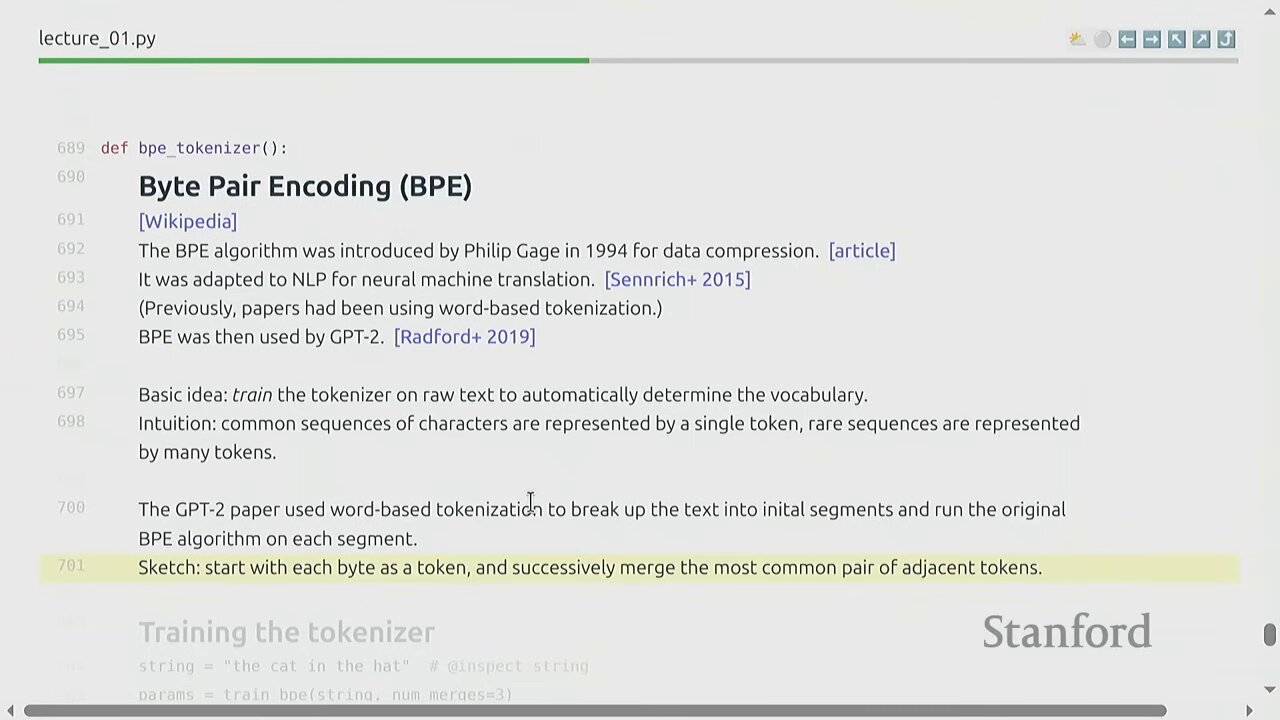
\includegraphics[width=\textwidth]{figures/fig_17_bpe_algorithm.jpg}
\caption{BPE 算法逐步演示：统计相邻对频次 $\to$ 合并最高频对 $\to$ 重复\protect\footnotemark}
\end{figure}
\footnotetext{视频画面时间区间：00:73:00--00:73:30。}

\textbf{预处理}：先按 word-based 方式把文本切成 segments（GPT-2 的 pre-tokenizer），再对每个 segment 独立跑 BPE。

\textbf{训练算法}（以 "cat and hat" 为例）：

\begin{enumerate}
\item 把字符串转成字节序列，如 $[99, 97, 116, 32, 97, 110, 100, 32, 104, 97, 116]$
\item 统计所有\textbf{相邻字节对}的频次
\item 找出频次最高的一对（如 $t,h \to [116, 104]$，出现 2 次）
\item 分配新 vocab 槽位：256（因为 0--255 已被原始字节占用）
\item 在序列中把 $[116, 104]$ 替换成 256
\end{enumerate}

重复以上步骤直到完成 $N_{\text{merges}}$ 次合并。

\begin{importantbox}{关键性质}
每轮序列长度\textbf{缩短}——压缩比越来越好，vocab 越来越大。这是一种用 vocab 空间换序列长度的交易。
\end{importantbox}

形式化地，设初始字节序列为 $\mathbf{x} = (x_1, x_2, \ldots, x_L)$，每轮 merge 操作定义为：

\[
\text{merge}(\mathbf{x}, (a, b) \to c) = \text{将所有相邻的 } (a,b) \text{ 替换为 } c
\]

其中 $c$ 是新分配的 vocab ID（从 256 开始递增）。

每轮选择合并哪一对的判据是频次最大化：

\[
(a^*, b^*) = \arg\max_{(a,b)} \sum_{i=1}^{|\mathbf{x}|-1} \mathbb{1}[x_i = a \wedge x_{i+1} = b]
\]

\begin{itemize}
\item $(a^*, b^*)$：本轮选中的最优合并对
\item $\mathbb{1}[\cdot]$：指示函数，条件满足时为 1，否则为 0
\item 每轮合并后序列长度减少 $\text{count}(a^*, b^*)$ 个元素
\end{itemize}

压缩比（compression ratio）定义为：

\[
r = \frac{\text{原始字节数}}{\text{token 数}} = \frac{L_{\text{bytes}}}{L_{\text{tokens}}}
\]

GPT-2 tokenizer 的压缩比约为 $r \approx 1.6$，意味着平均每个 token 代表 1.6 个字节。压缩比越高，序列越短，attention 的 $O(N^2)$ 计算量就越小。

\subsection{Encode 与 Decode}

\textbf{Encode}（推理时用）：输入新字符串，转字节，然后\textbf{按训练时 merges 的顺序}依次应用每个 merge，输出整数序列。

\begin{warningbox}{Percy 提示的优化点}
朴素实现遍历所有 merges，但应该只遍历\textbf{相关的} merges。这是 A1 性能优化点之一。
\end{warningbox}

\textbf{Decode}：输入整数序列，反查 vocab（整数 $\to$ 字节），拼接字节，UTF-8 解码，输出原始字符串。

\subsection{为什么 BPE 赢了}

\begin{figure}[H]
\centering
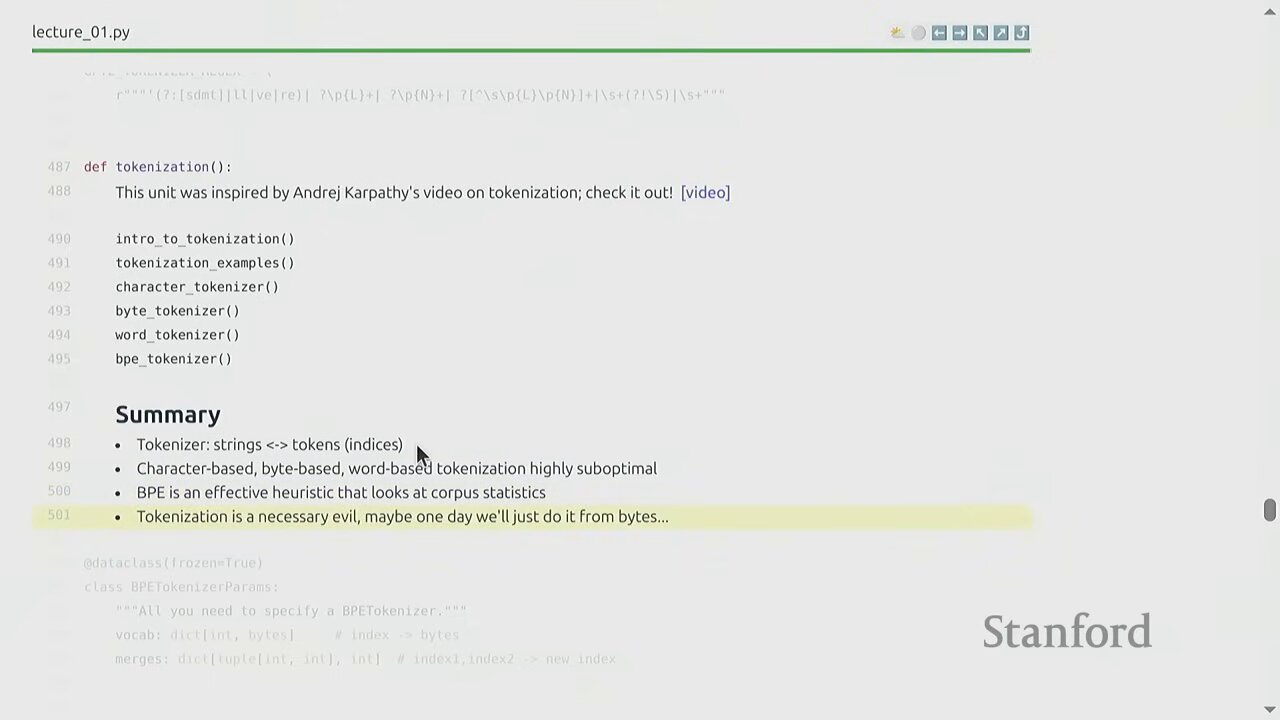
\includegraphics[width=\textwidth]{figures/fig_18_bpe_summary.jpg}
\caption{四种分词方案的对比总结\protect\footnotemark}
\end{figure}
\footnotetext{视频画面时间区间：00:77:20--00:77:50。}

\begin{tabular}{p{2cm}p{1.5cm}p{1.5cm}p{1.5cm}p{1.8cm}p{2.5cm}}
\toprule
\textbf{维度} & \textbf{Character} & \textbf{Byte} & \textbf{Word} & \textbf{BPE} & \\
\midrule
Vocab 大小 & 巨大 & 256（太小） & 无界 & \textbf{可控} & \\
压缩比 & 差 & 1.0（差） & 好 & \textbf{好（自适应）} & \\
稀疏问题 & 严重 & 无 & 严重（UNK） & \textbf{无} & \\
可逆 & ✅ & ✅ & ❌ & \textbf{✅} & \\
自适应 & ❌ & ❌ & ❌ & \textbf{✅} & \\
\bottomrule
\end{tabular}

\vspace{0.3cm}

BPE 是当前的最佳实践，因为它是唯一同时满足\textbf{可控 vocab、高压缩比、无稀疏、可逆、自适应}五个条件的方案。

\begin{knowledgebox}{Percy 的结语}
"我希望有一天不用再讲这堂课——因为那时我们有直接处理字节的架构了。在那之前，我们还得跟分词打交道。"这指向了一个开放问题：能否设计一种架构，直接在字节上高效运作，绕过分词？

字符级方案的问题可以用信息论视角理解。Unicode 有超过 14 万个码点，但大多数极其罕见。均匀分配 vocab 名额给每个码点，违反了信息论中的"高频短编码"原则。香农熵告诉我们，最优编码长度应与出现概率的对数反相关：

\[
\ell_i^* \approx -\log_2 p(x_i)
\]

\begin{itemize}
\item $\ell_i^*$：字符 $x_i$ 的最优编码长度（比特）
\item $p(x_i)$：字符 $x_i$ 在语料中的出现概率
\item 字符级方案给所有字符分配相同的"vocab 名额"（1 个 token），无视频率差异
\end{itemize}

BPE 虽然不是直接优化信息熵，但它通过频率驱动的 merge 操作，隐式地实现了这种自适应编码：高频序列获得更短的 token 表示，低频序列则被拆解为更基本的单元。
\end{knowledgebox}

\subsection{本章小结}

分词是字符串与整数序列的双向映射。四种方案中，BPE 凭借语料统计驱动的自适应合并机制胜出。BPE 训练通过反复合并最高频相邻对来构建 vocab，encode 时按训练顺序 replay merges，decode 反查 vocab 即可。

\section{总结与延伸}

\subsection{核心论点}

\begin{importantbox}{四个核心论点}
\begin{enumerate}
\item \textbf{从零构建是理解的前提}：LLM 的抽象层是 leaky 的，基础研究必须拆栈。这是课程存在的根本理由。
\item \textbf{效率是统一主线}：compute-constrained regime 下，从数据过滤到架构选择，每个决策都是效率驱动的。
\item \textbf{小模型学机制和心态，直觉只能学一半}：但 2.5/3 已物超所值。不要因为 representative gap 就否定小模型的价值。
\item \textbf{BPE 是当前的效率妥协}：优雅的字节级方案在当前 $O(N^2)$ attention 架构下太慢。BPE 是工程上的最优解。
\end{enumerate}
\end{importantbox}

\subsection{下节预告}

Lecture 2 将深入 PyTorch 的构建块，并进行 \textbf{Resource Accounting}——精确追踪每一份 FLOPs 去了哪里。这是 Systems 模块的基础。

\subsection{配套阅读}

以下论文已预存于 Readwise（tag \texttt{cs336/a1}），建议按 assignment 进度阅读：

\begin{tabular}{p{7cm}p{6cm}}
\toprule
\textbf{论文} & \textbf{对应知识点} \\
\midrule
Attention Is All You Need (Vaswani 2017) & Transformer 基础 \\
RoFormer: Rotary Position Embedding (Su 2021) & RoPE \\
Layer Normalization (Ba 2016) & LayerNorm $\to$ RMSNorm \\
Adam (Kingma 2014) & 优化器基础 \\
Decoupled Weight Decay / AdamW (Loshchilov 2017) & AdamW \\
TinyStories (Eldan 2023) & A1 训练数据 \\
\bottomrule
\end{tabular}

%% --- 正文内容结束 ---

\end{document}
